\documentclass[11pt,a4paper]{article}

\usepackage[margin=2.3cm]{geometry}
\IfFileExists{lmodern.sty}{\usepackage[T1]{fontenc}\usepackage{lmodern}}{}
\usepackage{amsmath,amssymb,amsthm,mathtools,bm}
\usepackage{booktabs,array,tabularx}
\usepackage{graphicx}
\usepackage{xcolor}
\usepackage{enumitem}
\usepackage{microtype}
\usepackage{tikz}
\usetikzlibrary{arrows.meta,positioning,calc,decorations.pathmorphing}
\usepackage[font=small,labelfont=bf]{caption}
\usepackage{hyperref}
\usepackage{cleveref}

\hypersetup{colorlinks=true,linkcolor=blue!55!black,citecolor=blue!55!black,urlcolor=blue!55!black}
\setlist{itemsep=2pt,topsep=4pt}

% ------------------------------------------------------------------ macros
\newcommand{\bq}{\bm q}
\newcommand{\bk}{\bm k}
\newcommand{\bp}{\bm p}
\newcommand{\bG}{\bm G}
\newcommand{\bK}{\bm K}
\newcommand{\br}{\bm r}
\newcommand{\eps}{\varepsilon}
\newcommand{\ii}{\mathrm i}
\newcommand{\dd}{\mathrm d}
\newcommand{\Tr}{\operatorname{Tr}}
\newcommand{\Ree}{\operatorname{Re}}
\newcommand{\Imm}{\operatorname{Im}}
\newcommand{\diag}{\operatorname{diag}}
\newcommand{\csch}{\operatorname{csch}}
\newcommand{\nF}{n_{\rm F}}
\newcommand{\nB}{n_{\rm B}}
\newcommand{\SigR}{\Sigma^{\rm R}}
\newcommand{\WR}{W^{\rm R}}
\newcommand{\ket}[1]{|#1\rangle}
\newcommand{\bra}[1]{\langle #1|}
\newcommand{\braket}[2]{\langle #1|#2\rangle}
\newcommand{\codeinner}[1]{\begingroup\small\ttfamily\def\_{\textunderscore\allowbreak}#1\endgroup}
\newcommand{\code}[1]{\ifmmode\text{\codeinner{#1}}\else\codeinner{#1}\fi}
\emergencystretch=3em
\newcommand{\dsum}{\textstyle\sum}

\newtheorem{assumption}{Assumption}
\theoremstyle{remark}
\newtheorem*{remark}{Remark}

\title{\textbf{Layer-resolved G$_0$W self-energy of van der Waals heterostructures\\ and the quantum-twisting-microscope conductance}\\[4pt]
\large Theory and implementation notes for the \texttt{g0w\_heterostructure} package}
\author{}
\date{\today}

\begin{document}
\maketitle

\begin{abstract}
These notes document, in a self-contained way, the physics and the numerics implemented in the
\texttt{g0w} package: the layer-resolved Coulomb kernel of $N$ two-dimensional sheets in a stratified,
possibly gated and dispersive dielectric; the random-phase-approximation (RPA) dielectric matrix and
screened interaction of a stack of decoupled electronic subsystems; the one-shot G$_0$W
(correlation) self-energy in the full-frequency and plasmon-pole forms, including its band-matrix
generalisation for multiband samples; the Dyson equation and the electronic spectral function; and the
differential conductance of a quantum twisting microscope (QTM) in the limit of a monolayer-graphene tip
with a small Fermi surface. Two samples are worked out in detail: doped monolayer graphene
(SLG\,$|$\,hBN\,$|$\,SLG) and twisted bilayer graphene (SLG tip\,$|$\,hBN\,$|$\,TBG). Every equation is
followed by the name of the function that implements it, and every approximation is listed explicitly.
\end{abstract}

\tableofcontents
\newpage

% ======================================================================
\section{Overview}
\label{sec:overview}
% ======================================================================

\subsection{What is computed}

The package computes the single-particle spectral function of the electrons of a two-dimensional
\emph{sample} embedded in an arbitrary van der Waals stack, dressed by the dynamically screened Coulomb
interaction at the level of one-shot G$_0$W, and the momentum-resolved tunneling conductance that a
quantum twisting microscope (QTM) measures on it. The chain of quantities is shown in \cref{fig:pipeline}:
\begin{enumerate}
\item the \textbf{bare Coulomb kernel} $V_{\ell\ell'}(q,\omega)$ between the $N$ sheets of the stack, from
      Poisson's equation in a stratified uniaxial dielectric with optional gates (\cref{sec:electrostatics});
\item the \textbf{electronic model} of every subsystem: bands $\xi_{n\bk}$, Bloch states and the
      layer-projected density matrix elements (form factors) $\rho^\ell_{nm}(\bk,\bq)$ (\cref{sec:models});
\item the \textbf{independent-particle polarisability} $\chi^0_{\ell\ell'}(\bq,\omega)$, the RPA dielectric
      matrix $\varepsilon=1-V\chi^0$ and the \textbf{screened interaction} $W=\varepsilon^{-1}V$, its spectral
      density $S$, the loss function and the collective modes (\cref{sec:screening});
\item the \textbf{retarded G$_0$W self-energy} $\Sigma_{nn'}(\bk,\eps)$ of the sample (\cref{sec:selfenergy});
\item the \textbf{spectral function} $A_{nn'}(\bk,\eps)$ from the Dyson equation (\cref{sec:spectral});
\item the \textbf{QTM differential conductance} $dI/dV(V,\theta)$ and $d^2I/dV^2$ (\cref{sec:qtm}).
\end{enumerate}
The results of the worked examples (notebooks 01--05) are collected in \cref{sec:results} and interpreted in
\cref{sec:interpretation} (notebook 06); grids, cost, validation and limitations are in \cref{sec:numerics}.

\begin{figure}[t]
\centering
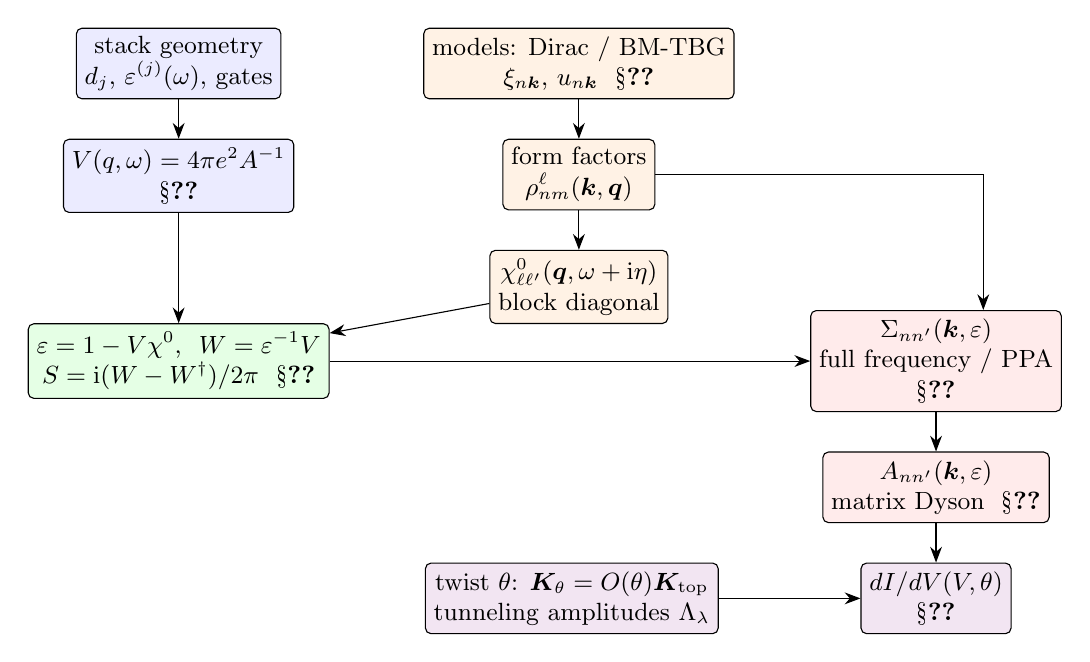
\begin{tikzpicture}[node distance=5mm and 7mm, every node/.style={font=\small},
  box/.style={draw, rounded corners=2pt, align=center, inner sep=3pt, fill=#1},
  box/.default={gray!8}, >={Stealth[length=2mm]}]
\node[box=blue!8] (geo) {stack geometry\\ $d_j$, $\varepsilon^{(j)}(\omega)$, gates};
\node[box=blue!8, below=of geo] (V) {$V(q,\omega)=4\pi e^2A^{-1}$\\ \S\ref{sec:electrostatics}};
\node[box=orange!10, right=18mm of geo] (H) {models: Dirac / BM-TBG\\ $\xi_{n\bk}$, $u_{n\bk}$ \ \S\ref{sec:models}};
\node[box=orange!10, below=of H] (rho) {form factors\\ $\rho^\ell_{nm}(\bk,\bq)$};
\node[box=orange!10, below=of rho] (chi) {$\chi^0_{\ell\ell'}(\bq,\omega+\ii\eta)$\\ block diagonal};
\node[box=green!10, below=of V, yshift=-9mm] (W) {$\varepsilon=1-V\chi^0$, \ $W=\varepsilon^{-1}V$\\ $S=\ii(W-W^\dagger)/2\pi$ \ \S\ref{sec:screening}};
\node[box=red!8, anchor=west] (Sig) at ($(W.east -| chi.east)+(18mm,0)$) {$\Sigma_{nn'}(\bk,\eps)$\\ full frequency / PPA\\ \S\ref{sec:selfenergy}};
\node[box=red!8, below=of Sig] (A) {$A_{nn'}(\bk,\eps)$\\ matrix Dyson \ \S\ref{sec:spectral}};
\node[box=violet!10, below=of A] (G) {$dI/dV(V,\theta)$\\ \S\ref{sec:qtm}};
\node[box=violet!10, left=18mm of G] (tw) {twist $\theta$: $\bK_\theta=O(\theta)\bK_{\rm top}$\\ tunneling amplitudes $\Lambda_\lambda$};
\draw[->] (geo) -- (V); \draw[->] (H) -- (rho); \draw[->] (rho) -- (chi);
\draw[->] (V) -- (W); \draw[->] (chi) -- (W);
\draw[->] (W.east) -- (Sig.west); \draw[->] (rho.east) -| ($(Sig.north)+(0.6,0)$);
\draw[->] (Sig) -- (A); \draw[->] (A) -- (G); \draw[->] (tw) -- (G);
\end{tikzpicture}
\caption{Computational chain. Blue: electrostatics of the stack; orange: electronic structure of the
subsystems; green: RPA screening; red: G$_0$W self-energy and spectral function; violet: QTM.}
\label{fig:pipeline}
\end{figure}

\subsection{Units and conventions}

\begin{center}
\begin{tabularx}{\textwidth}{lX}
\toprule
quantity & convention\\
\midrule
energies, frequencies, temperature & eV, with $\hbar=k_B=1$ \\
lengths, momenta & nm, nm$^{-1}$\\
electrostatics & Gaussian: $\nabla\cdot(\bm\varepsilon\nabla\phi)=-4\pi\rho$, $e^2=1.4399764$ eV\,nm\\
2D Fourier transforms & $f(\bq)=\int\dd^2r\,e^{-\ii\bq\cdot\br}f(\br)$; $V(q)$ in eV\,nm$^2$\\
momentum integrals & $\frac1A\sum_{\bq}\to\int\frac{\dd^2q}{(2\pi)^2}$; weights $w_{\bq}$ in nm$^{-2}$\\
response & retarded, evaluated at $\omega+\ii\eta$, $\eta>0$\\
dielectric matrix & $\varepsilon=1-V\chi^0$ \quad(\emph{not} $1-\chi^0V$)\\
screened interaction & $W=\varepsilon^{-1}V$ \quad(\emph{not} $V\varepsilon^{-1}$)\\
spectral density of $W$ & $S=\ii(W-W^\dagger)/(2\pi)$, $=-\Imm W/\pi$ for symmetric $W$\\
energies of states & $\xi_{n\bk}=E_{n\bk}-\mu$ (measured from the sample Fermi level)\\
spectral function & $A=\ii(G-G^\dagger)/(2\pi)$, $\int A\,\dd\eps=1$ per state\\
twist rotation & $O(\theta)=\begin{psmallmatrix}\cos\theta&\sin\theta\\-\sin\theta&\cos\theta\end{psmallmatrix}$ (clockwise, as in Ref.~\cite{Wei2025})\\
flattened index & $(\ell,\bG)\mapsto \ell\,n_G+G$ for every matrix in (layer, reciprocal-vector) space\\
\bottomrule
\end{tabularx}
\end{center}

\subsection{Physical assumptions}
\label{sec:assumptions}

The following assumptions are made throughout; where they are relaxed or tested this is said explicitly.

\begin{assumption}[Electrostatics]\label{as:electro}
The sheets are infinitely thin and the Coulomb interaction is quasi-static (no retardation:
$q\gg\omega/c$). Each dielectric region is homogeneous, local and uniaxial with the optical axis along $z$,
$\bm\varepsilon=\diag(\varepsilon_\parallel,\varepsilon_\parallel,\varepsilon_z)$, possibly dispersive and
lossy. Gates are grounded perfect conductors.
\end{assumption}

\begin{assumption}[Decoupled subsystems]\label{as:decoupled}
Different electronic subsystems (e.g.\ the QTM tip and the sample) are not tunnel coupled when the
screening is computed: there is no density operator connecting them, so $\chi^0$ is block diagonal and all
inter-subsystem physics is in $V$. Within a subsystem (the two layers of TBG) the layers are hybridised by
the electronic Hamiltonian and $\chi^0$ has layer-off-diagonal elements.
\end{assumption}

\begin{assumption}[RPA and one-shot G$_0$W]\label{as:gw}
The density response is the RPA one built on the bare (or Hartree) bands, and the self-energy is the first
term of Hedin's equations, $\Sigma=\ii G_0W_0$, with the non-interacting $G_0$ of the sample. Vertex
corrections and self-consistency are neglected. Only the \emph{correlation} part
$\Sigma_c=\ii G_0(W-V)$ is kept; the bare exchange (Fock) term is excluded (\cref{sec:exchange}).
\end{assumption}

\begin{assumption}[Head only]\label{as:head}
Unless stated otherwise only the $\bG=\bG'=0$ (head) element of the moir\'e reciprocal-lattice structure of
$\chi^0$, $W$ and of the form factors is kept (local-field effects off, $n_G=1$).
\end{assumption}

\begin{assumption}[Weak tunneling and small tip Fermi surface]\label{as:qtm}
Tip--sample tunneling is treated to lowest order and conserves in-plane momentum; the tip is a non-interacting
graphene sheet whose chemical potential follows the bias while its bands stay fixed relative to the sample Fermi
level; the sample chemical potential does not move relative to the sample bands; the tip Fermi momentum is small
compared with the momentum scale on which the sample spectral function varies; $T=0$ (finite $T$ by smoothing).
Only elastic tunneling into the dressed sample states is included (interactions enter through $A^S$)~\cite{Wei2025}.
\end{assumption}

\subsection{Package layout}

\begin{center}
\small
\begin{tabularx}{\textwidth}{lX}
\toprule
module & content\\
\midrule
\code{g0w.layer\_coulomb} & $V(q,\omega)$ of $N$ sheets; gates; capped slab; branch-tracked $\kappa(\omega)$ (\S\ref{sec:electrostatics})\\
\code{g0w.dielectrics} & hBN, SiO$_2$, Al$_2$O$_3$ dielectric functions\\
\code{g0w.layer\_helpers} & \code{layer\_helpers\_G}, \code{LayerHelpers}: $\rho^\ell_{nm}$, $\chi^0$, $\varepsilon$, loss from \texttt{pybandstructure}\\
\code{g0w.screening} & block-diagonal $\chi^0$, $\varepsilon$ and $W$ of a stack, loss, layer-channel split\\
\code{g0w.self\_energy\_ppa} & plasmon poles and residues, PPA self-energy, $q$ weights\\
\code{g0w.self\_energy\_full\_frequency} & full-frequency $\Sigma$, band-matrix $\Sigma_{nn'}$, resolvent kernels\\
\code{g0w.spectral} & scalar/matrix Dyson equation, $A$, quasiparticle solution\\
\code{g0w.qtm} & twist kinematics, tunneling amplitudes, $dI/dV$, $d^2I/dV^2$ (SLG and TBG)\\
\code{g0w.models.dirac\_chi} & analytic $\chi^0$ of doped graphene\\
\code{g0w.models.slg\_stack}, \code{slg\_self\_energy} & SLG$|$hBN$|$SLG junction, Dirac form factor, $\Sigma$, $A$\\
\code{g0w.models.tbg\_model}, \code{tbg\_stack}, \code{tbg\_self\_energy} & TBG continuum model, three-sheet stack, $\Sigma_{nn'}$\\
\code{g0w.satellites} & satellite energies: emission edge, energy-loss decomposition of $-\Imm\Sigma$ (\S\ref{sec:interpretation})\\
\code{notebooks/01}--\code{06} & executed examples: geometry, SLG G$_0$W, TBG G$_0$W, QTM on SLG and on TBG, satellites\\
\code{scripts/run\_slg\_qtm.py}, \code{run\_tbg\_qtm.py} & command-line drivers for the $dI/dV$ maps (\code{.npz} + \code{.png})\\
\code{tests/} & regression and physics tests (\code{python tests/run\_tests.py})\\
\bottomrule
\end{tabularx}
\end{center}

% ======================================================================
\section{Electrostatics of the stack: the layer-resolved Coulomb kernel}
\label{sec:electrostatics}
% ======================================================================

\subsection{Geometry}

$N$ sheets $\ell=0,\dots,N-1$ sit at heights $z_0>z_1>\dots>z_{N-1}$ and divide space into $N+1$ regions
(\cref{fig:stack}): region $0$ above sheet $0$, region $j$ ($1\le j\le N-1$) between sheets $j-1$ and $j$,
of thickness $d_{j-1}=z_{j-1}-z_j$ (\code{d[j-1]} in the code), and region $N$ below sheet $N-1$. The outer
regions are half-spaces, or are terminated by grounded gates at distances $d_{\rm t}$ above sheet $0$ and
$d_{\rm b}$ below sheet $N-1$ (\code{top\_gate\_d}, \code{bottom\_gate\_d}), or (top only) by a slab of
thickness $d_{\rm s}$ backed by a half-space $\varepsilon_{\rm c}$ (\code{CappedLayerCoulomb}).

\begin{figure}[h]
\centering
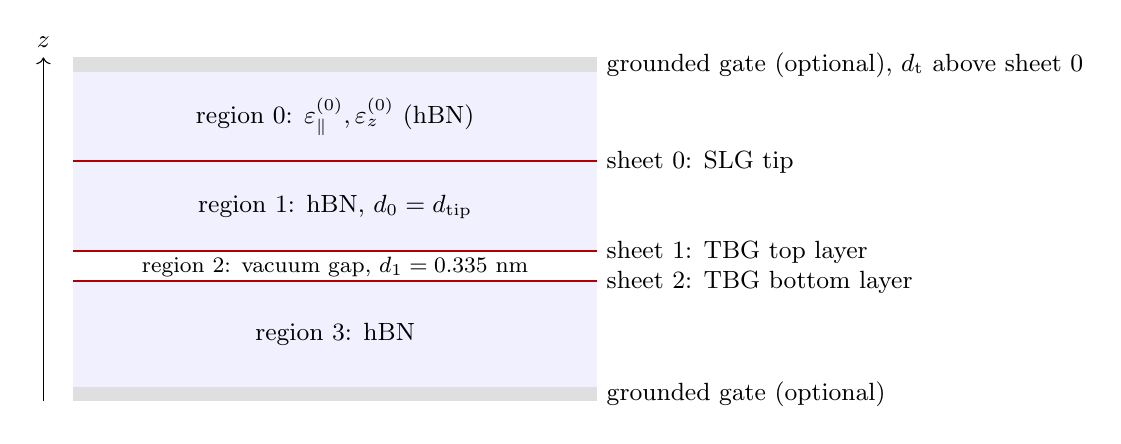
\begin{tikzpicture}[scale=0.95, every node/.style={font=\small}]
\fill[gray!25] (0,4.4) rectangle (7,4.6); \node[right] at (7,4.5) {grounded gate (optional), $d_{\rm t}$ above sheet 0};
\fill[blue!6] (0,3.2) rectangle (7,4.4); \node at (3.5,3.8) {region 0: $\varepsilon^{(0)}_\parallel,\varepsilon^{(0)}_z$ (hBN)};
\draw[very thick, red!70!black] (0,3.2) -- (7,3.2); \node[right] at (7,3.2) {sheet 0: SLG tip};
\fill[blue!6] (0,2.0) rectangle (7,3.2); \node at (3.5,2.6) {region 1: hBN, $d_0=d_{\rm tip}$};
\draw[very thick, red!70!black] (0,2.0) -- (7,2.0); \node[right] at (7,2.0) {sheet 1: TBG top layer};
\fill[white] (0,1.6) rectangle (7,2.0); \node at (3.5,1.8) {\footnotesize region 2: vacuum gap, $d_1=0.335$ nm};
\draw[very thick, red!70!black] (0,1.6) -- (7,1.6); \node[right] at (7,1.6) {sheet 2: TBG bottom layer};
\fill[blue!6] (0,0.2) rectangle (7,1.6); \node at (3.5,0.9) {region 3: hBN};
\fill[gray!25] (0,0.0) rectangle (7,0.2); \node[right] at (7,0.1) {grounded gate (optional)};
\draw[->] (-0.4,0) -- (-0.4,4.6) node[above] {$z$};
\end{tikzpicture}
\caption{The three-sheet stack used for the TBG sample (notebooks 03, 05). For SLG$|$hBN$|$SLG there are two
sheets and three hBN regions.}
\label{fig:stack}
\end{figure}

\subsection{Poisson equation in one region}

With $\bm E=-\nabla\phi$, $\bm D=\bm\varepsilon\bm E$ and $\nabla\cdot\bm D=4\pi\rho$, a 2D Fourier transform
in the plane gives, inside region $j$ (no free charge),
\begin{equation}
\varepsilon_z^{(j)}\partial_z^2\phi-\varepsilon_\parallel^{(j)}q^2\phi=0
\quad\Rightarrow\quad
\phi''=\kappa_j^2\phi,\qquad
\kappa_j=q\sqrt{\varepsilon_\parallel^{(j)}/\varepsilon_z^{(j)}},\qquad
Y_j=\varepsilon_z^{(j)}\kappa_j=q\sqrt{\varepsilon_\parallel^{(j)}\varepsilon_z^{(j)}} .
\label{eq:kappaY}
\end{equation}
$Y_j$ is the \emph{admittance} of the region (\code{compute\_kappa\_Y}). For a spacer of thickness $d$
whose lower and upper faces are at potentials $\Phi_b$ and $\Phi_a$, the solution
$\phi(z)=[\Phi_a\sinh\kappa z+\Phi_b\sinh\kappa(d-z)]/\sinh\kappa d$ ($0\le z\le d$) gives the normal
displacement on the two faces:
\begin{equation}
\varepsilon_z\phi'(d^-)=Y\bigl[\Phi_a\coth\kappa d-\Phi_b\csch\kappa d\bigr],\qquad
\varepsilon_z\phi'(0^+)=Y\bigl[\Phi_a\csch\kappa d-\Phi_b\coth\kappa d\bigr].
\label{eq:spacer}
\end{equation}
For a half-space above sheet $0$, $\phi=\Phi_0e^{-\kappa(z-z_0)}$ and $\varepsilon_z\phi'=-Y_0\Phi_0$; with a
grounded gate at distance $d_{\rm t}$, $\phi=\Phi_0\sinh\kappa(z_{\rm g}-z)/\sinh\kappa d_{\rm t}$ and
$\varepsilon_z\phi'=-Y_0\coth(\kappa d_{\rm t})\,\Phi_0$. A gate therefore replaces the boundary admittance
$Y\to Y\coth(\kappa d_{\rm g})$, which tends to $Y$ for $d_{\rm g}\to\infty$. A slab
$(\kappa_s,Y_s,d_s)$ capped by a half-space with $Y_c=\varepsilon_cq$ gives instead
\begin{equation}
Y_{\rm eff}=Y_s\,\frac{Y_c+Y_s\tanh\kappa_sd_s}{Y_s+Y_c\tanh\kappa_sd_s},
\label{eq:capped}
\end{equation}
which interpolates between $Y_c$ ($d_s\to0$), $Y_s$ ($d_s\to\infty$) and the gate result ($Y_c\to\infty$)
(\code{capped\_slab\_admittance}).

\subsection{Matching at the sheets: the tridiagonal admittance matrix}

The potential is continuous across sheet $\ell$ and the displacement jumps by the sheet charge,
$D_z(z_\ell^+)-D_z(z_\ell^-)=4\pi\sigma_\ell$, i.e.\
$-\varepsilon_z\phi'(z_\ell^+)+\varepsilon_z\phi'(z_\ell^-)=4\pi\sigma_\ell$. Inserting \cref{eq:spacer} for
the regions above (region $\ell$) and below (region $\ell+1$) sheet $\ell$:
\begin{equation}
\bigl[Y_\ell\coth\kappa_\ell d_{\ell-1}+Y_{\ell+1}\coth\kappa_{\ell+1}d_\ell\bigr]\Phi_\ell
-Y_\ell\csch(\kappa_\ell d_{\ell-1})\,\Phi_{\ell-1}
-Y_{\ell+1}\csch(\kappa_{\ell+1}d_\ell)\,\Phi_{\ell+1}=4\pi\sigma_\ell ,
\end{equation}
with the outermost terms replaced by the boundary admittances ($Y_0$, $Y_0\coth\kappa_0d_{\rm t}$ or
$Y_{\rm eff}$ on top; $Y_N$ or $Y_N\coth\kappa_Nd_{\rm b}$ at the bottom). This is
$A(q,\omega)\Phi=4\pi\sigma$ with a tridiagonal $A$ (\code{build\_tridiagonal\_A\_diagonals}):
\begin{align}
A_{00}&=Y_{\rm top}+Y_1\coth\kappa_1d_0, &
A_{N-1,N-1}&=Y_{N-1}\coth\kappa_{N-1}d_{N-2}+Y_{\rm bot},\nonumber\\
A_{\ell\ell}&=Y_\ell\coth\kappa_\ell d_{\ell-1}+Y_{\ell+1}\coth\kappa_{\ell+1}d_\ell, &&\nonumber\\
A_{\ell,\ell-1}&=-Y_\ell\csch\kappa_\ell d_{\ell-1}, &
A_{\ell,\ell+1}&=-Y_{\ell+1}\csch\kappa_{\ell+1}d_\ell .
\label{eq:Amatrix}
\end{align}
A unit point charge $e$ on sheet $m$ has $\sigma_\ell(\bq)=e\,\delta_{\ell m}$, and the energy of a second
charge $e$ on sheet $\ell$ is $e\Phi_\ell$. The layer-resolved Coulomb kernel is therefore
\begin{equation}
\boxed{V_{\ell m}(q,\omega)=4\pi e^2\,[A^{-1}(q,\omega)]_{\ell m}}
\qquad[\text{eV\,nm}^2]
\label{eq:V}
\end{equation}
(\code{LayerCoulomb.coulomb\_matrix}). $A$ is inverted with a Thomas LU factorisation and $\coth$, $\csch$
are evaluated in the overflow-safe form $\coth z=(1+u)/(1-u)$, $\csch z=2e^{-z}/(1-u)$, $u=e^{-2z}$, with
$1-u=-\mathrm{expm1}(-2z)$.

\paragraph{Closed forms (tested).} A single sheet in a uniform medium has $A=2\varepsilon q$, i.e.\
$V=2\pi e^2/(\varepsilon q)$; with gates at $\pm d$, $V=\frac{2\pi e^2}{\varepsilon q}\tanh qd$; with one gate,
$V=\frac{2\pi e^2}{\varepsilon q}(1-e^{-2qd})$. Two sheets in a uniform uniaxial medium:
\begin{equation}
V_{11}=V_{22}=\frac{2\pi e^2}{\bar\varepsilon q},\qquad V_{12}=V_{11}\,e^{-\kappa d},
\qquad \bar\varepsilon=\sqrt{\varepsilon_\parallel\varepsilon_z},\quad\kappa=q\sqrt{\varepsilon_\parallel/\varepsilon_z}.
\label{eq:bilayerV}
\end{equation}

\subsection{Bilayer channels and the effect of gates}
\label{sec:channelsV}

For two equivalent sheets, $V$ is diagonalised by $u_\pm=(1,\pm1)/\sqrt2$ with eigenvalues
$V_\pm=V_{11}\pm V_{12}$. At $qd\ll1$, $V_+\simeq 4\pi e^2/(\bar\varepsilon q)$ (the total charge sees the
long-range Coulomb field) while $V_-\simeq V_{11}\kappa d=2\pi e^2 d/\varepsilon_z$ is finite (a dipole layer).
$V_+$ drives the in-phase (optical, $\omega\propto\sqrt q$) plasmon and $V_-$ the out-of-phase (acoustic,
$\omega\propto q$) plasmon. Gates at distance $d_{\rm g}$ cut the long-range part,
$V_+\to 4\pi e^2 d_{\rm g}/\varepsilon_z$ for $qd_{\rm g}\ll1$ (gates at $\pm d_{\rm g}$), but leave $V_-$ almost unchanged when
$d\ll d_{\rm g}$: gating raises the \emph{relative} weight of the acoustic channel by suppressing the optical one
(notebook 01, test \code{test\_gate\_suppresses\_in\_phase\_more\_than\_out\_of\_phase}).

\subsection{Dispersive dielectrics and passivity}

hBN is modelled with one Lorentz oscillator per axis,
\begin{equation}
\varepsilon_\alpha(\omega)=\varepsilon_{\infty,\alpha}+\frac{\varepsilon_{0,\alpha}-\varepsilon_{\infty,\alpha}}{1-\omega^2/\omega_{T,\alpha}^2-\ii\gamma_\alpha\omega/\omega_{T,\alpha}^2},
\end{equation}
with $(\varepsilon_0,\varepsilon_\infty,\omega_T,\gamma)=(6.41,4.53,168,0.82)$ (in-plane) and
$(3.0,2.5,94.2,0.23)$ (out-of-plane), energies in meV (\code{dielectrics.HBNModel}). Between $\omega_T$ and
$\omega_L=\omega_T\sqrt{\varepsilon_0/\varepsilon_\infty}$ (the Reststrahlen bands, 94--103 meV and
168--200 meV) $\varepsilon_\parallel\varepsilon_z<0$ and $\kappa$ is almost imaginary: the substrate carries
hyperbolic phonon polaritons and $V$ acquires a large dissipative part. For the retarded kernel of a passive
medium the anti-Hermitian part must be negative semidefinite, $-(V-V^\dagger)/2\ii\succeq0$. The branch of
$\kappa_j(\omega)$ is the decaying one ($\Ree\kappa>0$) at the first frequency of a sweep and is then
continued without jumps (\code{compute\_kappa\_Y\_tracked}); in the examples of notebook 01 the continued
and the principal branches coincide and both are passive. Static values ($\omega\to0$) are used unless the
phonon range is of interest (all calculations in notebooks 02--05).

% ======================================================================
\section{Electronic models}
\label{sec:models}
% ======================================================================

\subsection{Doped monolayer graphene}
\label{sec:slgmodel}

Near one Dirac point, $h(\bp)=\hbar v_F(\tau p_x\sigma_x+p_y\sigma_y)$ with $\bp$ measured from the Dirac
point, $\hbar v_F=0.658$ eV\,nm ($v_F=10^6$ m/s) and $g=g_sg_v=4$. The bands and spinors are
\begin{equation}
\xi^s_{\bp}=s\hbar v_F|\bp|-E_F,\qquad u^s_{\bp}=\tfrac{1}{\sqrt2}(1,\,s\,e^{\ii\phi_{\bp}}),\qquad s=\pm1,
\end{equation}
with $k_F=\sqrt{4\pi n/g}$ and $E_F=\hbar v_Fk_F$ ($n=10^{12}$ cm$^{-2}$ $\Rightarrow$ $k_F=0.1772$ nm$^{-1}$,
$E_F=116.6$ meV). The overlap that dresses every Coulomb vertex is the chirality factor
\begin{equation}
F^{s's}(\bp,\bp')=|\braket{u^{s'}_{\bp}}{u^{s}_{\bp'}}|^2=\tfrac12\bigl[1+ss'\cos\angle(\bp,\bp')\bigr],
\qquad \textstyle\sum_sF^{s's}=1,
\label{eq:chirality}
\end{equation}
which forbids intraband backscattering and interband forward scattering
(\code{slg\_self\_energy.make\_dirac\_form\_factor}). The sample has only one sheet, so the layer-projected
form factor is $\rho^\ell=\delta_{\ell S}\braket{u}{u'}$: a sample electron has no intermediate state in the tip.

\subsection{Twisted bilayer graphene: continuum model}
\label{sec:tbgmodel}

\paragraph{Hamiltonian.} One valley ($\tau=+$) of the Bistritzer--MacDonald model in the form of
Koshino \emph{et al.}~\cite{BM2011,Koshino2018} as implemented in \texttt{pybandstructure}
(\code{koshino}). In the basis of plane waves $\bk+\bG$ ($\bG$ in the moir\'e reciprocal lattice,
$|\bG|\le G_{\max}|\bG_M|$, $G_{\max}=3$, i.e.\ 37 shells) and of the four orbitals
$(\ell,\sigma)\in\{t,b\}\times\{A,B\}$,
\begin{gather}
H_{\bG\bG'}(\bk)=\delta_{\bG\bG'}
\begin{pmatrix}h_t(\bk+\bG)&0\\0&h_b(\bk+\bG)\end{pmatrix}
+\sum_{j=1}^3\Bigl[\delta_{\bG-\bG',\bm g_j}\begin{pmatrix}0&T_j\\0&0\end{pmatrix}+{\rm h.c.}\Bigr],
\nonumber\\
h_\ell(\bk)=\hbar v\,\bigl[R_\ell(\bk-\bK_\ell)\bigr]\cdot(\tau\sigma_x,-\sigma_y),
\end{gather}
where $R_{t,b}=O(\pm\theta_{\rm TBG}/2)$, $\bK_{1,2}=\frac{|\bG_M|}{\sqrt3}(-\frac{\sqrt3}{2},\pm\frac12)$ are the
moir\'e $\kappa$ points at which the top ($1$) and bottom ($2$) Dirac cones sit, $\bm g_j\in\{0,\bm b_1,\bm b_2\}$
and $T_j=u_{AA}\sigma_0+u_{AB}(\ldots)$ are the three interlayer hoppings with
$|\bG_M|=8\pi\sin(\theta_{\rm TBG}/2)/(\sqrt3a)$, $a=0.246$ nm. Parameters (Ref.~\cite{Wei2025}):
$\theta_{\rm TBG}=1.20^\circ$, $u_{AB}=117$ meV, $u_{AA}=0.7u_{AB}$, $\hbar v=0.657$ eV\,nm, so that
$\alpha=u_{AB}/(\hbar vk_\theta)=0.56$ and the two central bands are 24--25 meV wide and separated from the
remote bands by $\approx44$ meV. Only the $2n_b=8$ bands closest to neutrality are computed
(\code{TBGParams.n\_bands}$=4$). The electrostatic environment differs from Ref.~\cite{Wei2025}, which uses an
isotropic background $\varepsilon_r=10$: here the TBG sits in anisotropic hBN,
$(\varepsilon_\parallel,\varepsilon_z)=(6.41,3)$, with vacuum between its layers (\code{TBGSLGConfig.eps\_par},
\code{eps\_z}, \code{eps\_interlayer}), so plasmon energies are not expected to coincide with that reference.

\paragraph{Model frame vs lab frame.} The model momentum $\bk$ is measured from the moir\'e $\gamma$ point.
The graphene (lab) momentum of the plane wave $\bk+\bG$ in either layer is
\begin{equation}
\bp=\bk+\bG+\bm\Gamma^{\rm lab},\qquad \bK^{\rm lab}_{\rm top}=\bm\Gamma^{\rm lab}+\bK_1,\quad
\bK^{\rm lab}_{\rm bot}=\bm\Gamma^{\rm lab}+\bK_2,
\label{eq:labframe}
\end{equation}
where $\bm\Gamma^{\rm lab}$ (\code{gamma\_point\_tblg}) lies on the $x$ axis and $|\bK^{\rm lab}_{\rm top,bot}|=4\pi/3a$
at angles $\pm\theta_{\rm TBG}/2$ (\code{tbg\_model.model\_frame}; checked in
\code{test\_model\_frame\_dirac\_points}, where the decoupled model has a zero-energy top-layer state at $\bK_1$).
This relation is what the QTM kinematics needs (\cref{sec:qtmtbg}).

\paragraph{Bloch states.} $H(\bk)u_{n\bk}=E_{n\bk}u_{n\bk}$ with components
$u_{n\bk}[4g+2\ell+\sigma]$, $g$ the plane-wave index. The states are stored once
(\code{band\_structure.wavefunctions}) and the \emph{same} gauge is used for the form factors, the self-energy
and the tunneling amplitudes. The chemical potential is fixed by the filling at temperature $T=5$ K
(charge neutrality by default); $\xi_{n\bk}=E_{n\bk}-\mu$.

\paragraph{Layer-resolved form factors.} The density of layer $\ell$ at momentum $\bq+\bG$,
$\rho_\ell(\bq+\bG)=\sum_{\bk}c^\dagger_{\bk}P_\ell e^{-\ii(\bq+\bG)\cdot\br}c_{\bk+\bq}$, has Bloch matrix elements
\begin{equation}
\rho^\ell_{nm}(\bk,\bq;\bG)=\bra{u_{n\bk}}P_\ell\,\hat\tau_{\bG}\ket{u_{m,\bk+\bq}}
\qquad(\code{densityL[l, n, m, k, q, G]}),
\label{eq:formfactor}
\end{equation}
where $P_\ell$ projects on the two sublattices of layer $\ell$ and $\hat\tau_{\bG}$ shifts the plane-wave
index; $\bk+\bq$ is folded back onto the mesh (\code{k\_plus\_q\_ind}) and the corresponding shift of the
plane-wave components is applied by \texttt{pybandstructure}. Completeness:
$\sum_\ell\rho^\ell_{nm}(\bk,0;0)=\delta_{nm}$ (\code{test\_density\_matrix\_completeness}).
Only $\bG=0$ is used for $\Sigma$ (\cref{as:head}).

\paragraph{Doping and Hartree.} For a doped sample the first-shell Hartree potential
$V_H=\sum_{|\bG|=G_M}\frac{2\pi e^2}{\varepsilon_H|\bG|}\delta n(\bG)e^{\ii\bG\cdot\br}$ can be solved
self-consistently (\code{tbg\_model.apply\_hartree}, needs the development version of \texttt{pybandstructure});
the densities $\delta n(\bG)$ are measured from charge neutrality (regularised occupations), and
$G_0$ is then built on the Hartree bands. At neutrality the Hartree potential of the BM model vanishes.

\subsection{Moir\'e Brillouin-zone meshes}

$\bk$ and $\bq$ run over the same $N_s\times N_s$ Wigner--Seitz mesh (\code{n\_sites}), with weights summing to one
and area $A_{\rm BZ}=\frac{\sqrt3}{2}|\bG_M|^2$; the 2D measure is
\begin{equation}
\int\frac{\dd^2q}{(2\pi)^2}f(\bq)\simeq\sum_{\bq}w_{\bq}f(\bq),\qquad w_{\bq}=\frac{A_{\rm BZ}}{(2\pi)^2}\,\text{weight}(\bq)
\qquad(\code{q\_weights\_from\_band\_structure}),
\label{eq:qweights}
\end{equation}
\emph{without} the spin--valley degeneracy (see \cref{sec:degeneracy}); $\bq=0$ is removed ($V$ diverges and its
measure vanishes). The band structure is computed for valley $K$; valley $K'$ follows by time reversal
(\cref{sec:valleys}).

% ======================================================================
\section{Screening: polarisability, dielectric matrix and screened interaction}
\label{sec:screening}
% ======================================================================

\subsection{Independent-particle polarisability}

For a subsystem with Bloch states $\ket{n\bk}$ the layer-resolved Lindhard function is
\begin{equation}
\chi^0_{\ell\ell'}(\bq,\omega)=\frac{g}{A}\sum_{\bk,n,m}
\frac{\nF(\xi_{n\bk})-\nF(\xi_{m,\bk+\bq})}{\omega+\ii\eta+\xi_{n\bk}-\xi_{m,\bk+\bq}}\;
\rho^\ell_{nm}(\bk,\bq)\,\bigl[\rho^{\ell'}_{nm}(\bk,\bq)\bigr]^*
\qquad[\text{nm}^{-2}\,\text{eV}^{-1}],
\label{eq:chi0}
\end{equation}
the response of the density of layer $\ell$ to a potential acting on layer $\ell'$. It is negative at
$\omega=0$ ($\chi^0\to-D(E_F)$ for $q\to0$ in a metal), retarded ($\Imm\chi^0_{\ell\ell}\le0$ for
$\omega>0$) and, for the head ($\bG=\bG'=0$), a $2\times2$ matrix for TBG
(\code{LayerHelpers.chi0\_block}, \code{tbg\_model.chi0\_tbg}). The degeneracy $g=4$ counts spin and valley.
The fast kernel evaluates \cref{eq:chi0} for all $(\ell,\bG,\ell',\bG')$ at once as a matrix product over the
transitions with $\nF(\xi_{n\bk})\neq\nF(\xi_{m\bk+\bq})$, and agrees with \texttt{pybandstructure}'s
\code{polarization} to $3\times10^{-15}$.

For graphene the $T=0$ bubble is known in closed form~\cite{Wunsch2006} (\cref{app:dirac},
\code{dirac\_chi.chi\_dirac\_phys}); it is written with the split root $\sqrt{z-1}\sqrt{z+1}$, analytic in the upper
half plane, and evaluated at complex $\omega+\ii\eta$. A charge-neutral tip contributes only the interband part
$\chi^0=-\frac{g}{16}\frac{q^2}{\sqrt{(\hbar v_Fq)^2-(\omega+\ii\eta)^2}}$ (no Drude weight).

\paragraph{Both valleys of TBG.}\label{sec:valleys}
The continuum model is diagonalised for valley $K$ only; write $X(\bq)=g\chi^K(\bq)$ for the bubble
\eqref{eq:chi0} of that valley multiplied by $g=4$. Time reversal maps valley $K$ at $\bk$ onto $K'$ at $-\bk$,
$E_{K'}(\bk)=E_K(-\bk)$ and $u_{K'}(\bk)=u_K(-\bk)^*$; inserted in \eqref{eq:chi0} this gives
$\chi^{K'}_{ab}(\bq)=\chi^{K}_{ba}(-\bq)$. The physical (spin $\times$ valley) response is therefore
\begin{equation}
\chi^0_{\rm TBG}(\bq,\omega)=\tfrac{g}{2}\bigl[\chi^K(\bq,\omega)+\chi^K(-\bq,\omega)^T\bigr]
=\tfrac12\bigl[X(\bq,\omega)+X(-\bq,\omega)^T\bigr]
\label{eq:valleysym}
\end{equation}
(\code{tbg\_model.chi0\_tbg}), as in Ref.~\cite{Wei2025}, where the RPA polarisation sums over both valleys
related by time reversal. It satisfies the Onsager relation $\chi^0(\bq)=\chi^0(-\bq)^T$, hence $W(\bq)=W(-\bq)^T$,
which is also what allows the frequency integral of the self-energy to be folded onto $\omega>0$
(\cref{sec:sigma_derivation}). Both terms are needed: the bands of a single valley are not inversion symmetric,
$E_K(\bk)\neq E_K(-\bk)$, so $X(\bq)$ alone is not time-reversal symmetric at finite $\bq$ (its long-wavelength
static limit is valley-even). On the few Wigner--Seitz boundary points where $-\bq$ is stored as $-\bq+\bG_0$, the
head at the stored representative is used (same $|\bq|$). The Onsager relation then holds on the whole mesh to
round-off (notebook 03, \code{test\_valley\_symmetrized\_chi0\_is\_time\_reversal\_symmetric}).

\paragraph{Block-diagonal $\chi^0$ of a stack.} For decoupled subsystems (\cref{as:decoupled})
\begin{equation}
\chi^0(\bq,\omega)=\begin{pmatrix}\chi^0_{\rm tip}(|\bq|,\omega)&0\\0&\chi^0_{\rm TBG}(\bq,\omega)\end{pmatrix}
\qquad(3\times3,\ \code{screening.assemble\_chi0}).
\end{equation}
The tip is unstructured on the moir\'e scale: its response depends on $|\bq|$ only and has no umklapp.

\subsection{Dielectric matrix and screened interaction}

The total potential acting on the electrons is the external one plus the Hartree potential of the induced
density, $\phi=\phi_{\rm ext}+V\delta n$ with $\delta n=\chi^0\phi$. Hence $\phi=\varepsilon^{-1}\phi_{\rm ext}$ with
\begin{equation}
\boxed{\varepsilon(\bq,\omega)=1-V(\bq,\omega)\,\chi^0(\bq,\omega)}
\qquad\text{and}\qquad
\boxed{W(\bq,\omega)=V+V\chi^0W=\varepsilon^{-1}(\bq,\omega)\,V(\bq,\omega)} ,
\label{eq:epsW}
\end{equation}
matrices in sheet space (and in $(\ell,\bG)$ space with local fields, $V_{(\ell\bG),(\ell'\bG')}=V_{\ell\ell'}(|\bq+\bG|)\delta_{\bG\bG'}$).
The product order matters: $V$ and $\chi^0$ do not commute, so $\varepsilon^{-1}V\ne V\varepsilon^{-1}$.
Both $V$ and $\chi^0$ are evaluated at $\omega+\ii\eta$ with the \emph{same} $\eta$
(\code{screening.screened\_interaction}, \code{tbg\_stack.build\_stack\_eps\_W},
\code{slg\_stack.stack\_eps\_and\_V}): an undamped collective mode then appears in $-\Imm W$ as a Lorentzian of
width $\simeq\eta$ that a finite frequency grid can integrate, instead of a $\delta$ function.

\subsection{Spectral density, loss function and passivity}
\label{sec:spectraldensity}

$W$ is analytic in the upper half plane and its dynamical part $W-V$ decays at large $|\omega|$. Its spectral
representation is
\begin{equation}
W(\bq,z)=V(\bq)+\int_{-\infty}^{\infty}\dd\nu\,\frac{S(\bq,\nu)}{z-\nu},\qquad
S(\bq,\nu)=\frac{\ii}{2\pi}\bigl[W(\bq,\nu+\ii0)-W(\bq,\nu+\ii0)^\dagger\bigr],
\label{eq:spectralrep}
\end{equation}
with $S(\bq,-\nu)=-S(-\bq,\nu)^{T}$. For a passive medium $S$ is Hermitian and positive semidefinite at $\nu>0$
(it is the absorption of the stack). When $W$ is a symmetric matrix, as for reciprocal systems,
$S=-\Imm W/\pi$ element by element (\code{spectral\_density\_matrix(W, hermitian=False)}). The Hermitian form is
used by default because it makes the causality of $\Sigma$ manifest (\cref{sec:passivity}); for the stacks considered here $W$ is symmetric to
$\lesssim10^{-10}$ and the two coincide. The \emph{loss function} of a set of sheets is
$L(\bq,\omega)=-\Imm\Tr_{\rm sheets}W(\bq,\omega)\ge0$; its peaks locate collective modes but also inherit every
structure of $\Imm\chi^0$, so they are a display tool, not a mode criterion.

\subsection{Collective modes and plasmon-pole data}
\label{sec:ppa}

Collective modes are zeros of $\varepsilon$: they are located as prominent minima of $|\lambda_{\min}(\varepsilon(\bq,\omega))|$
on the real axis (prominence filter against continuum ripples, \code{find\_plasmon\_poles\_at\_q}). Around each
pole $\omega_n(\bq)$ the residue \emph{matrix} of $W$ is
\begin{equation}
R_n(\bq)=\int_{\omega_n-\Delta_-}^{\omega_n+\Delta_+}\dd\omega\;S(\bq,\omega),
\label{eq:residue}
\end{equation}
integrated over a window of $\pm5\eta$ truncated at the mid-points between neighbouring poles and, optionally,
on a refined local grid (\code{build\_plasmon\_pole\_data(eps\_builder=..., n\_refine=129)}). $R_n$ is Hermitian
PSD; a window of $\pm5\eta$ captures $\frac{2}{\pi}\arctan5\simeq87\%$ of a Lorentzian. The plasmon-pole
approximation (PPA) replaces $S(\bq,\omega)\to\sum_nR_n(\bq)\delta(\omega-\omega_n(\bq))$ for $\omega>0$. The
fraction of $\int S$ captured by the poles measures its validity; in doped graphene above $q\simeq k_F$ and
in TBG at small $q$ the modes are Landau damped and most of the weight is in the continuum, so the PPA is
used only as a diagnostic and the production route is the full-frequency one.

\subsection{Layer-symmetry channels}
\label{sec:channels}

For a pair of sheets $(a,b)$ write the $2\times2$ block of $W$ with $P_\pm=u_\pm u_\pm^T$,
$u_\pm=(1,\pm1)/\sqrt2$:
\begin{equation}
W_{\rm block}=\underbrace{P_+WP_+}_{\text{in phase}}+\underbrace{P_-WP_-}_{\text{out of phase}}
+\underbrace{P_+WP_-+P_-WP_+}_{\text{cross}} .
\label{eq:channels}
\end{equation}
This is an identity, exact and additive, and since $\Sigma$ is linear in $S$ the split carries over to the
self-energy (\code{screening.split\_layer\_channels}, \code{slg\_self\_energy.sigma\_full\_frequency\_channels\_kernel}).
For two equivalent sheets $u_\pm$ are exact eigenvectors of $W$ and the cross term vanishes; the in-phase and
out-of-phase parts are the optical and acoustic plasmon channels. It is a symmetry projection, valid also where
the modes are damped and are not poles. Whether the out-of-phase part is a second mode or the same mode
re-weighted by geometry must be checked from the peak positions of the two channels (with an inert tip both
peak at the same $\omega$).

% ======================================================================
\section{The G$_0$W self-energy}
\label{sec:selfenergy}
% ======================================================================

\subsection{Derivation}
\label{sec:sigma_derivation}

In the band basis of the sample, the first-order (GW) self-energy at the fermionic Matsubara frequency
$\ii\omega_n$ is (Hedin~\cite{Hedin1965}, Mahan~\cite{Mahan})
\begin{equation}
\Sigma_{nn'}(\bk,\ii\omega_n)=-\frac1\beta\sum_{\ii\Omega_m}\int\!\frac{\dd^2q}{(2\pi)^2}\sum_m\sum_{ab}
\rho^a_{nm}(\bk,\bq)\,W_{ab}(\bq,\ii\Omega_m)\,\bigl[\rho^b_{n'm}(\bk,\bq)\bigr]^*\,
G^0_m(\bk+\bq,\ii\omega_n+\ii\Omega_m),
\label{eq:sigma_matsubara}
\end{equation}
with $G^0_m(\bk,z)=1/(z-\xi_{m\bk})$, $a,b$ running over the sheets of the sample (the tip is not an
intermediate state, \cref{as:decoupled}) and $\rho$ the form factors \eqref{eq:formfactor}. (With $W\to V$ and
the convergence factor $e^{\ii\Omega0^+}$ this is the Fock term $-\int_{\bq}V\,\nF(\xi_{m\bk+\bq})|\rho|^2$.)
Split $W=V+W_c$ and use the spectral representation \eqref{eq:spectralrep},
$W_c(\bq,\ii\Omega)=\int\dd\nu\,S(\bq,\nu)/(\ii\Omega-\nu)$. The bosonic sum is done by contour integration,
\begin{equation}
\frac1\beta\sum_{\ii\Omega_m}\frac{1}{(\ii\Omega_m-\nu)(\ii\Omega_m+\ii\omega_n-\xi)}
=-\frac{\nB(\nu)+\nF(\xi)}{\ii\omega_n+\nu-\xi},
\end{equation}
using $\nB(\xi-\ii\omega_n)=-\nF(\xi)$. After the analytic continuation $\ii\omega_n\to\eps+\ii0^+$, the
correlation self-energy is
\begin{equation}
\Sigma^{c}_{nn'}(\bk,\eps)=\int\!\frac{\dd^2q}{(2\pi)^2}\sum_m\sum_{ab}\rho^a_{nm}\,[\rho^b_{n'm}]^*
\int_{-\infty}^{\infty}\!\dd\nu\;S_{ab}(\bq,\nu)\,\frac{\nB(\nu)+\nF(\xi_m)}{\eps+\nu-\xi_m+\ii0^+},
\qquad\xi_m\equiv\xi_{m,\bk+\bq},
\label{eq:sigma_full_line}
\end{equation}
which is Eqs.~(37) and (39) of Ref.~\cite{Wei2025} with the layer index in place of the moir\'e $\bG$ index.
Using $S(\bq,-\nu)=-S(-\bq,\nu)^T$ (\cref{eq:spectralrep}) together with the Onsager relation
$S(-\bq,\nu)^T=S(\bq,\nu)$ of a time-reversal-symmetric sample (\cref{sec:valleys}), i.e.\ $S(\bq,-\nu)=-S(\bq,\nu)$,
and $\nB(-\nu)=-1-\nB(\nu)$, the negative frequencies are folded onto $\nu>0$:
\begin{equation}
\boxed{\Sigma_{nn'}(\bk,\eps)=-\sum_{\bq}w_{\bq}\sum_m\sum_{ab}\rho^a_{nm}(\bk,\bq)\bigl[\rho^b_{n'm}(\bk,\bq)\bigr]^*
\int_0^{\omega_{\max}}\!\dd\omega\;S_{ab}(\bq,\omega)\,\mathcal D_m(\omega,\eps)}
\label{eq:sigma}
\end{equation}
\begin{equation}
\mathcal D_m(\omega,\eps)=\frac{A^+_m(\omega)}{\omega+\xi_m-\eps-\ii\eta_\Sigma}+\frac{A^-_m(\omega)}{-\omega+\xi_m-\eps-\ii\eta_\Sigma},
\qquad A^\pm_m=\nB(\omega)+\nF(\mp\xi_m)\ \xrightarrow{T=0}\ \Theta(\pm\xi_m).
\label{eq:D}
\end{equation}
The first term describes an electron in an empty state ($\xi_m>0$) of energy $\eps=\xi_m+\omega$ that has emitted
a boson of energy $\omega$; the second a hole ($\xi_m<0$) at $\eps=\xi_m-\omega$. $\eta_\Sigma$ is a small
broadening of the resolvents (the $0^+$). \Cref{eq:sigma} is implemented in
\begin{itemize}
\item \code{compute\_self\_energy\_band\_matrix} (TBG, band matrix, direct frequency contraction) and
      \code{compute\_self\_energy\_band\_matrix\_kernel} (same, fast route, \cref{sec:kernel});
\item \code{compute\_self\_energy\_full\_frequency\_pybandstructure} (TBG, diagonal $n=n'$, returned in the layer basis
      as the Hadamard product $\rho^a\rho^{b*}\circ\int S\mathcal D$, whose sum over $(a,b)$ is $\Sigma_{nn}$);
\item \code{slg\_self\_energy.sigma\_full\_frequency\_fast}, \code{sigma\_full\_frequency\_kernel} (graphene,
      radial $q$ grid with angular average, \cref{sec:radial}).
\end{itemize}

\subsection{Causality}
\label{sec:passivity}

The anti-Hermitian part of \cref{eq:sigma} is, for $\eta_\Sigma\to0$,
\begin{equation}
\frac{\Sigma-\Sigma^\dagger}{2\ii}=-\pi\sum_{\bq}w_{\bq}\sum_m\Bigl[A^+_m\,R_m S(\bq,\eps-\xi_m)R_m^\dagger
+A^-_m\,R_mS(\bq,\xi_m-\eps)R_m^\dagger\Bigr],\qquad (R_m)_{na}=\rho^a_{nm}(\bk,\bq),
\end{equation}
a sum of negative semidefinite matrices when $S\succeq0$ and $A^\pm\ge0$. Hence $\Imm\Sigma_{nn}\le0$ and the
spectral function below is positive. This holds exactly with the Hermitian spectral density and is verified
numerically (\code{spectral.is\_passive}).

\subsection{Momentum integration}
\label{sec:radial}

\paragraph{Moir\'e mesh (TBG).} $\bq$ runs over the full 2D mesh with the weights \eqref{eq:qweights}; the
direction of $\bq$ is part of the sum and $\bk+\bq$ is folded onto the same mesh, so the external $\bk$ must be a
mesh point. Removing $\bq=0$ is harmless: the integrand vanishes as $q\to0$ because
$\int\dd^2q\,V(q)\sim\int q\,\dd q/q$ is finite.

\paragraph{Radial grid (isotropic samples).} For graphene $S(\bq,\omega)$ depends on $|\bq|$ only, and the 2D
measure is split as
\begin{equation}
\int\frac{\dd^2q}{(2\pi)^2}f(\bk,\bq)=\int_0^{q_{\max}}\frac{q\,\dd q}{2\pi}\,\bigl\langle f(\bk,\bq(\vartheta))\bigr\rangle_\vartheta,
\qquad\langle\cdot\rangle_\vartheta=\frac1{2\pi}\int_0^{2\pi}\dd\vartheta ,
\label{eq:radial}
\end{equation}
trapezoidal weights $w_q=q\Delta q/2\pi$ (\code{make\_radial\_q\_weights}) and $n_\vartheta=64$ uniform angles
(\code{make\_angular\_quadrature}). The angular average must be done: the intermediate energy
$\xi^s_{\bk-\bq}=s\hbar v_F|\bk-\bq|-E_F$ and the chirality factor depend on $\vartheta$. Sampling only
$\vartheta=0$ (collinear) is a different quantity, not a coarse approximation. Defaults: $q\in[0.02,3]k_F$
($n_q=96$), $\omega\in(0,2.8E_F]$ ($n_\omega=480$).

\subsection{Spin and valley degeneracy}
\label{sec:degeneracy}

The polarisation bubble \eqref{eq:chi0} sums over the $g=4$ flavours of the particle--hole pair, so $g$ enters
$\chi^0$, $\varepsilon$ and $W$. In \cref{eq:sigma_matsubara} the internal electron line carries the flavour of
the external electron (the Coulomb vertex conserves spin and, for $|\bq|\ll|\bK|$, valley), so there is no free
flavour sum and \emph{no} degeneracy factor in $w_{\bq}$; including one would make $\Sigma$ four times too large.
Spin and valley enter the self-energy only through the screening of $W$.

\subsection{What is not included: exchange and double counting}
\label{sec:exchange}

Only the correlation part is computed: $S$ is the spectral density of $W$, and $\Imm V=0$ for a static
background, so the bare-exchange (Fock) self-energy
$\Sigma^x_{nn'}=-\sum_{\bq}w_{\bq}\sum_m\nF(\xi_m)\sum_{ab}\rho^a_{nm}V_{ab}(\bq)[\rho^b_{n'm}]^*$ is absent.
$\Sigma^x$ is real and static: it shifts and reshapes the quasiparticle bands but cannot produce satellites or
lifetimes. Ref.~\cite{Wei2025} (Sec.~IV\,B) likewise neglects the first-order Hartree and Fock diagrams for
this reason, and the Coulomb interaction is normal ordered. The consequences differ between the two samples:
\begin{itemize}
\item \textbf{TBG at neutrality.} The Hartree potential of the BM model vanishes at neutrality, while the Fock term
would renormalise the flat bands. The correlation-only $\Sigma$ is the self-energy of the
scheme of Ref.~\cite{Wei2025}; positions of quasiparticle peaks are those of the bare continuum bands dressed
by $\Ree\Sigma_c$ only, which should be kept in mind when comparing with experiment.
\item \textbf{Doped graphene.} The omitted $\Sigma^x$ is what enhances the Fermi velocity of
graphene~\cite{Elias2011}. Without it the correlation part alone narrows the band
($v^*/v_F\simeq0.92$ in notebook 02). Since $\Sigma^x$ is real, it leaves $\Imm\Sigma$ and hence the energy of
the satellite structure unchanged, but it moves the quasiparticle peak by $\Sigma^x_{nn}(\bk)$ and thus changes
the offset between the two. Quasiparticle velocities and peak--satellite offsets of doped graphene computed
here are therefore correlation-only quantities; $\Sigma^x$ can be added to the Dyson equation as a static term
when needed.
\end{itemize}

\subsection{Plasmon-pole form}

Inserting $S\to\sum_nR_n\delta(\omega-\omega_n)$ in \cref{eq:sigma}:
\begin{equation}
\Sigma^{\rm PPA}_{nn'}(\bk,\eps)=-\sum_{\bq}w_{\bq}\sum_{m,p}\sum_{ab}\rho^a_{nm}[\rho^b_{n'm}]^*R_{p,ab}(\bq)\,
\mathcal D_m(\omega_p(\bq),\eps)
\end{equation}
(\code{compute\_self\_energy\_layer}, \code{compute\_self\_energy\_pybandstructure}). The full residue matrix is used;
a rank-one factorisation $R_p\simeq\Phi_p\Phi_p^\dagger$ is a diagnostic only.

\subsection{Fast route: tabulated resolvent kernels}
\label{sec:kernel}

In \cref{eq:sigma,eq:D} $\xi_m$ and $\eps$ appear in the resolvents only through $u=\xi_m-\eps$, while the
populations split as $A^\pm=\nB(\omega)+\nF(\mp\xi_m)$. Therefore
\begin{equation}
\int_0^{\omega_{\max}}\!\dd\omega\,S(\bq,\omega)\mathcal D_m(\omega,\eps)=\nF(-\xi_m)\,P_{\bq}(u)+\nF(\xi_m)\,M_{\bq}(u)+B^+_{\bq}(u)+B^-_{\bq}(u),
\label{eq:kernel}
\end{equation}
\begin{equation}
P_{\bq}(u)=\int\dd\omega\frac{S(\bq,\omega)}{\omega+u-\ii\eta_\Sigma},\quad
M_{\bq}(u)=\int\dd\omega\frac{S(\bq,\omega)}{-\omega+u-\ii\eta_\Sigma},\quad
B^\pm_{\bq}(u)=\int\dd\omega\frac{\nB(\omega)S(\bq,\omega)}{\pm\omega+u-\ii\eta_\Sigma}.
\end{equation}
These four matrix functions of one variable depend on $\bq$ only. They are tabulated once on a uniform $u$ grid
of spacing $\eta_\Sigma/8$ (with the same trapezoidal rule in $\omega$) and linearly interpolated for every
$(\bk,m,\eps)$ (\code{ResolventKernel}). This is an exact rewriting up to the interpolation error
($\lesssim2\times10^{-4}$ relative in the tests), and makes the cost per external $\bk$ independent of $n_\omega$:
for graphene it is $\sim300$ times faster than the direct contraction, which makes full twist maps cheap.
At $T=0$ the Bose terms vanish since the $\omega$ grid starts above zero.

\subsection{Numerical parameters and their roles}

\begin{center}
\small
\begin{tabularx}{\textwidth}{llX}
\toprule
symbol & code & role\\
\midrule
$\eta$ & \code{cfg.eta}, \code{TBGParams.eta} & broadening of $\chi^0$ and $V$ ($\omega+\ii\eta$); sets the width of undamped plasmons in $S$. TBG default: $2\hbar v^*|\bG_M|/N_s$ (mesh-tied, flat-band regime only)\\
$\eta_\Sigma$ & \code{eta\_self} & $0^+$ of the resolvents in \cref{eq:D}; floors $\Imm\Sigma$ near $\eps=0$ (the Fermi-liquid $\eps^2$ law is recovered only for $\eps\gg\eta_\Sigma$)\\
$\eta_{\rm qp}$ & \code{eta\_qp} & extrinsic width in the Dyson equation (finite junction, disorder); keeps the QP peak finite\\
$\omega_{\max}$, $n_\omega$ & \code{omega\_grid} & frequency window of $S$; must contain the plasmon branches and the relevant continuum\\
$q_{\max}$, $n_q$, $n_\vartheta$ & radial grid & graphene: $3k_F$, 96, 64 (convergence: $n_q$ is the slow one, $\sim1/n_q$)\\
$N_s$, $n_b$ & \code{n\_sites}, \code{n\_bands} & TBG mesh and number of bands per side; memory of \code{densityL} $\propto 2(2n_b)^2N_s^4$\\
\bottomrule
\end{tabularx}
\end{center}

% ======================================================================
\section{Dyson equation and spectral function}
\label{sec:spectral}
% ======================================================================

\subsection{Green's function and spectral function}

With the bare propagator $G^0(\bk,\eps)=\sum_n\ket{n\bk}\bra{n\bk}/(\eps+\ii\eta_{\rm qp}-\xi_{n\bk})$ and the
self-energy matrix of \cref{eq:sigma}, the Dyson equation $G=G^0+G^0\Sigma G$ restricted to a set of $n_b$
bands reads (Ref.~\cite{Wei2025}, Eq.~(50))
\begin{equation}
G(\bk,\eps)=\bigl[(\eps+\ii\eta_{\rm qp})\,\mathbb 1-\diag(\xi_{n\bk})-\Sigma(\bk,\eps)\bigr]^{-1},
\qquad
A(\bk,\eps)=\frac{\ii}{2\pi}\bigl[G(\bk,\eps)-G(\bk,\eps)^\dagger\bigr]
\label{eq:dyson}
\end{equation}
(\code{spectral.green\_function\_matrix}, \code{spectral\_function\_matrix}). $A$ is Hermitian and positive
semidefinite whenever $(\Sigma-\Sigma^\dagger)/2\ii\preceq0$ (\cref{sec:passivity}), because
$A=\frac1\pi G\,\Gamma\,G^\dagger$ with $\Gamma=\eta_{\rm qp}\mathbb1-(\Sigma-\Sigma^\dagger)/2\ii\succeq0$. Its trace
obeys $\int\dd\eps\,\Tr A=n_b$ (checked to $10^{-3}$ for $\Sigma=0$, \code{test\_spectral\_function\_normalised\_without\_interactions}).
If $\Sigma$ is diagonal (band-diagonal approximation, or exactly for isotropic graphene, where the chirality
structure makes $\Sigma$ diagonal in the band basis) this reduces to
\begin{equation}
A_n(\bk,\eps)=-\frac1\pi\Imm\frac{1}{\eps-\xi_{n\bk}-\Sigma_{nn}(\bk,\eps)+\ii\eta_{\rm qp}}
=\frac1\pi\,\frac{\eta_{\rm qp}-\Imm\Sigma_{nn}}{(\eps-\xi_{n\bk}-\Ree\Sigma_{nn})^2+(\eta_{\rm qp}-\Imm\Sigma_{nn})^2}
\label{eq:Ascalar}
\end{equation}
(\code{spectral.spectral\_function\_scalar}, \code{slg\_self\_energy.spectral\_function\_sample}). The band-off-diagonal
elements matter where two bands are close compared with $|\Sigma|$, e.g.\ inside the flat-band manifold of TBG,
where $\|\Sigma_{\rm off}\|/\|\Sigma_{\rm diag}\|\simeq0.3$ at $\kappa_{\rm top}$ (notebook 03). Within an exactly
degenerate pair of bands the split into diagonal and off-diagonal parts depends on the gauge, and only the
matrix (or a gauge-invariant contraction such as \cref{eq:didv}) is meaningful.

\subsection{Reading the spectral function}

\paragraph{Quasiparticle peak.} Near the solution $E^*_{n\bk}$ of
\begin{equation}
E^*-\xi_{n\bk}-\Ree\Sigma_{nn}(\bk,E^*)=0
\end{equation}
$A$ is a Lorentzian of weight and width
\begin{equation}
Z=\bigl[1-\partial_\eps\Ree\Sigma_{nn}\bigr]^{-1}_{E^*},\qquad \Gamma=2Z\bigl(\eta_{\rm qp}-\Imm\Sigma_{nn}(E^*)\bigr)
\end{equation}
(\code{spectral.quasiparticle\_solution}). The peak does not sit at the bare band: $\Ree\Sigma$ displaces it, and
the missing weight $1-Z$ is transferred to the incoherent part and to the satellites.

\paragraph{Satellites.} Away from the quasiparticle pole, to first order in $\Sigma$ (Ref.~\cite{Wei2025}, Eq.~(34)),
\begin{equation}
A_{\lambda_1\lambda_2}(\bk,\eps)\simeq-\frac1\pi\frac{\Sigma''_{\lambda_1\lambda_2}(\bk,\eps)}{(\eps-\xi_{\lambda_1\bk})(\eps-\xi_{\lambda_2\bk})},
\qquad \Sigma''=\frac{\Sigma-\Sigma^\dagger}{2\ii},
\end{equation}
so peaks of $-\Imm\Sigma$ produce satellites. From \cref{eq:sigma}, $-\Imm\Sigma$ is large where an electron at
$\eps$ can emit a boson: $\eps=\xi_{m\bk+\bq}+\omega$ with $S(\bq,\omega)$ large. A dispersionless mode of energy
$\omega_0$ (the flat-band plasmon of TBG) therefore gives a satellite at $\eps\simeq\xi_{\rm VH}+\omega_0$ where the
intermediate density of states peaks ($\xi_{\rm VH}$ the van Hove energy of the flat band), nearly independent of
$\bk$. For a dispersive mode (the $\sqrt q$ plasmon of graphene) the satellite sits at $\eps=\xi_{\bk-\bq}+\omega_{\bq}$
summed over $\bq$; since $\xi_{\bk-\bq}\ne\xi_{\bk}$, its offset from the quasiparticle peak is not the plasmon
energy at any single $\bq$; how to estimate it from the plasmon dispersion is shown in \cref{sec:edge}. For one-boson
emission the satellite lies on the side of the quasiparticle peak away from $E_F$ (above it for empty states,
below it for occupied ones).

\paragraph{Fermi-liquid region.} At $\eps\to0$, $-\Imm\Sigma\propto\eps^2$; on a numerical grid this is floored
by $\eta_\Sigma$ and by the finite $q$ mesh, so the region $|\eps|\lesssim20\eta_\Sigma$ is not physical.

% ======================================================================
\section{Quantum twisting microscope: differential conductance}
\label{sec:qtm}
% ======================================================================

In the QTM~\cite{Inbar2023} a graphene tip is pressed onto the sample through a thin hBN barrier and rotated by
an angle $\theta$; the tunneling current is recorded as a function of bias $V$ and $\theta$. Because tunneling
across a clean, flat interface conserves in-plane crystal momentum, the twist selects \emph{which momentum of the
sample} is probed, and the bias selects the energy: the $(\theta,V)$ map is a momentum- and energy-resolved
picture of the sample spectral function~\cite{Wei2025b,Wei2025}. This section derives the expression used by
\code{g0w.qtm} and describes the kinematics for the SLG and TBG samples.

\subsection{From the tunneling Hamiltonian to $dI/dV$}

\paragraph{Tunneling Hamiltonian.} Let $c_{\bk\sigma}$ annihilate a tip electron of lab momentum $\bk$ on sublattice
$\sigma$ and $d_{\bp\sigma'}$ a top-layer electron of the sample. For a junction of area $\Omega$ much larger than
the lattice constants, the tunneling amplitude conserves lab momentum modulo the reciprocal lattices of the two
crystals, $\bp+\bG_S=\bk+\bG_T$ with $\bG_T=O(\theta)\bG_S$ (Ref.~\cite{Wei2025}, Eq.~(30)); $O(\theta)$ is the
clockwise rotation $\bigl(\begin{smallmatrix}\cos\theta&\sin\theta\\-\sin\theta&\cos\theta\end{smallmatrix}\bigr)$
(\code{qtm.rotation\_matrix}). Its Fourier components fall off on the atomic scale, so only the processes with
$|\bk+\bG_T|\simeq|\bp+\bG_S|\simeq K=4\pi/3a$ survive: three Bragg channels $j=1,2,3$ linking the three
equivalent corners of the two Brillouin zones. In channel $j$ the sublattice structure is
$t^{(j)}_{\sigma\sigma'}=w\,e^{\ii(\bG^j_T\cdot\bm\tau_\sigma-\bG^j_S\cdot\bm\tau_{\sigma'})}$, and with the origin on
an atom the representative channel $j=1$ has all phases equal to one,
\begin{equation}
t^{(1)}=w\begin{pmatrix}1&1\\1&1\end{pmatrix}=w\,\ket{\chi}\bra{\chi},\qquad \ket\chi=(1,1)^T .
\label{eq:tunnelmatrix}
\end{equation}
For a $C_3$-symmetric sample the three channels probe $C_3$-related momenta with $C_3$-related matrix elements and
contribute equally (factor $N_b=3$). The tip couples only to the layer it touches (the top layer of TBG):
tunneling decays exponentially with distance.

\paragraph{Current.} To lowest order in $w$ (\cref{as:qtm}) the current from tip to sample is the golden-rule
expression
\begin{equation}
I=\frac{2\pi e}{\hbar}N_fN_b\sum_{\bk}\int\dd\eps\,
\bigl[\nF(\eps-\mu_T)-\nF(\eps-\mu_S)\bigr]\,
\Tr\bigl[t^{(1)\dagger}A_T(\bk,\eps)\,t^{(1)}A^{\rm top}_S(\bp(\bk),\eps)\bigr],
\label{eq:current}
\end{equation}
with $N_f=4$ spin--valley flavours, $A_T$ the $2\times2$ (sublattice) spectral function of the tip and
$A_S^{\rm top}$ the top-layer sublattice block of the sample spectral function at the conserved momentum
$\bp(\bk)$. Using \cref{eq:tunnelmatrix}, the trace factorises into $w^2\bra\chi A_T\ket\chi\,\bra\chi A^{\rm top}_S\ket\chi$.

\paragraph{Bias and the tip as a momentum filter.} Following Ref.~\cite{Wei2025}, (a) the tip is non-interacting
graphene, and its chemical potential follows the bias while its band energies stay fixed relative to the sample
Fermi level, $\partial(\xi^T+eV)/\partial V\simeq0$: the bias changes only the occupations in \cref{eq:current},
$\mu_T=\mu_S+eV$; (b) the sample chemical potential does not move relative to the sample bands (for TBG because
of the large flat-band density of states, for the doped SLG sample because it is fixed by its own gate);
(c) $T=0$. Differentiating \cref{eq:current} with respect to $V$ then gives
$dI/dV\propto\sum_{\bk}\Tr[t^{(1)\dagger}A_T(\bk,\mu_T)\,t^{(1)}A^{\rm top}_S(\bp(\bk),\mu_S+eV)]$: only tip states \emph{at the
tip Fermi level} contribute, and they lie on the tip Fermi line around the tip Dirac point
$\bK_\theta=O(\theta)\bK$. (d) The tip Fermi momentum is small, so that $A_S$ is constant along this line and is
evaluated at $\bp=\bK_\theta$. What remains of the tip is
$\sum_{\bk}\bra\chi A_T(\bk,\mu_T)\ket\chi=\Omega\,\nu_T\,\langle|\braket{\chi}{u_T}|^2\rangle=\Omega\,\nu_T$: the average of
$|1+se^{\ii\phi}|^2/2$ over the tip Fermi line equals one, so the tip spinor disappears and only the tip density of
states $\nu_T$ survives. The three Bragg channels do not interfere at generic (incommensurate) angles and add up
to the factor $N_b$. The result is (Ref.~\cite{Wei2025}, Eqs.~(8) and (33))
\begin{equation}
\boxed{\frac{dI}{dV}(V,\theta)=e^2\Gamma\sum_{\lambda\rho}\Lambda_\lambda(\bK_\theta)\,
A^S_{\lambda\rho}(\bK_\theta,eV)\,\Lambda_\rho(\bK_\theta)^*
=e^2\Gamma\,\bra{\chi_\theta}A^S(eV)\ket{\chi_\theta}},
\quad \Gamma=\tfrac{2\pi}{\hbar}w^2\Omega\,\nu_TN_bN_f
\label{eq:didv}
\end{equation}
($\Gamma$ of Ref.~\cite{Wei2025}, Eq.~(8), times $N_f$), where $eV$ is measured from $\mu_S$ and is the energy axis of $A^S$ (bias and
sample energy are the same axis: \code{eps\_values} = $eV$). The band-basis spectral function of
\cref{eq:dyson} enters through $A^{\rm top}_S=\sum_{\lambda\rho}\ket{u^{\rm top}_\lambda}A_{\lambda\rho}\bra{u^{\rm top}_\rho}$,
so the tunneling amplitude is the sublattice sum of the top-layer spinor of the Bloch state (Ref.~\cite{Wei2025}, Eq.~(32)),
\begin{equation}
\Lambda_\lambda(\bK_\theta)=\braket{\chi}{u^{\rm top}_{\lambda}(\bK_\theta)}=u^\lambda_{\bK_\theta,tA}+u^\lambda_{\bK_\theta,tB}.
\label{eq:Lambda}
\end{equation}
The code returns $dI/dV/(e^2\Gamma)$ in eV$^{-1}$ and drops $\Gamma$.

\paragraph{Properties.} (i) Positivity: $dI/dV=e^2\Gamma\bra{\chi_\theta}A^S\ket{\chi_\theta}\ge0$ because $A^S$ is PSD
(\cref{sec:spectral}). (ii) Gauge invariance: under $u_\lambda\to e^{\ii\varphi_\lambda}u_\lambda$,
$\Lambda_\lambda\to e^{\ii\varphi_\lambda}\Lambda_\lambda$ and $A_{\lambda\rho}\to e^{-\ii\varphi_\lambda}A_{\lambda\rho}e^{\ii\varphi_\rho}$,
so \cref{eq:didv} is invariant \emph{provided $\Lambda$ and $\Sigma$ are built from the same eigenvectors}
(\code{test\_band\_matrix\_didv\_is\_gauge\_invariant\_and\_positive}). With the band-diagonal approximation the off-diagonal terms are dropped and
only $|\Lambda_\lambda|^2$ enters, which is gauge invariant by itself. (iii) Non-interacting limit:
$dI/dV=\sum_\lambda|\Lambda_\lambda|^2\delta_{\eta}(eV-\xi_{\lambda\bK_\theta})$ (\code{tbg\_bare\_didv}).

\paragraph{What \cref{eq:didv} leaves out.} The radius of the tip Fermi line, $k_{F,T}$, sets the momentum
resolution, which \cref{eq:didv} treats as perfect. If the tip bands do move with the bias (a tip with fixed
doping, whose Dirac point follows $\mu_T$), the derivative of \cref{eq:current} acquires a second term from tip
states below the tip Fermi level, on rings $|\bk-\bK_\theta|=|\eps-E_{D,T}|/\hbar v$; it is dropped by
assumption (a). Self-energy effects of the tip, inelastic (boson-assisted) tunneling as a separate channel, and the
bias dependence of the electrostatics are not included: interactions enter only through the dressed sample
spectral function (\cref{as:qtm}), whose plasmon satellites are, in this language, the inelastic features.
At finite temperature \cref{eq:didv} is convolved with $-\partial_\eps\nF$, a bell of standard deviation
$\pi k_BT/\sqrt3\simeq1.8k_BT$ (0.8 meV at 5 K); \code{qtm.smooth\_bias} applies a Gaussian of chosen width,
which also mimics the lock-in modulation.

\subsection{SLG sample}
\label{sec:qtmslg}

Tip and sample are both graphene with Dirac point $\bK=(K,0)$ at $\theta=0$. Measured from the sample Dirac
point the probed momentum is (\code{qtm.slg\_probe\_momentum})
\begin{equation}
\bp_\theta=\bK_\theta-\bK=\bigl(O(\theta)-1\bigr)\bK,\qquad |\bp_\theta|=2K\sin\tfrac{\theta}{2}\simeq K\theta
=0.297\ \text{nm}^{-1}\ \text{per degree},
\label{eq:ptheta}
\end{equation}
almost perpendicular to $\bK$. One degree already corresponds to $1.7k_F$ at $n=10^{12}$ cm$^{-2}$. The isotropic
cone makes $\Sigma$ diagonal in the chirality basis (\cref{sec:spectral}), and with the spinor $(1,se^{\ii\phi_{\bp}})/\sqrt2$
\begin{equation}
\frac{dI}{dV}=e^2\Gamma\sum_{s=\pm}|\Lambda_s(\bp_\theta)|^2A^S_s(\bp_\theta,eV),\qquad
|\Lambda_s|^2=1+s\cos\phi_{\bp_\theta}
\label{eq:didvslg}
\end{equation}
(\code{qtm.slg\_spectral\_map}, \code{slg\_didv}). Since $\phi_{\bp_\theta}\simeq-\frac{\pi}{2}-\frac{\theta}{2}$,
$\cos\phi_{\bp_\theta}=-\sin\frac\theta2$ and the two bands are probed with nearly equal weight (difference
$<4\%$ for $\theta<2^\circ$); \code{tunneling\_model="constant"} sets $|\Lambda_s|^2=1$ and reads $A^S$ directly.
The map shows two quasiparticle ridges $eV=\pm\hbar v^*|\bp_\theta|-E_F$ (renormalised velocity $v^*$, \cref{sec:spectral})
and the plasmaron satellites displaced from them. The twist sets the \emph{external} momentum $\bp_\theta$; the
plasmon momentum is integrated over inside $\Sigma(\bp_\theta,\eps)$ and must not be confused with $\bp_\theta$.
The angle can be converted to momentum and back with \code{qtm.twist\_to\_momentum} and \code{momentum\_to\_twist}.

\subsection{TBG sample}
\label{sec:qtmtbg}

\paragraph{Kinematics.} Now $\theta$ is the twist between the tip and the \emph{top} layer of TBG, and the tip couples
to the top-layer plane-wave components. A top-layer plane wave $\bk+\bG$ of the continuum model carries the lab momentum
$\bk+\bG+\bm\Gamma^{\rm lab}$ (\cref{eq:labframe}). Momentum conservation with the tip Dirac point
$\bK^{\rm lab}_\theta=O(\theta)\bK^{\rm lab}_{\rm top}$ then fixes the extended-zone model momentum
\begin{equation}
\boxed{\bk_\theta=O(\theta)\,\bK^{\rm lab}_{\rm top}-\bm\Gamma^{\rm lab}}\qquad(\code{qtm.tbg\_tip\_momentum}),
\label{eq:ktheta}
\end{equation}
which passes through
\begin{equation}
\theta=0:\ \bk_\theta=\bK_1\ (\kappa_{\rm top}),\qquad
\theta=\theta_{\rm TBG}:\ \bk_\theta=\bK_2\ (\kappa_{\rm bot}),\qquad
\theta=-\theta_{\rm TBG}:\ \bk_\theta\simeq2\bK_1-\bK_2\ (\gamma'),
\end{equation}
the first two exactly (both Dirac points lie on the circle $|\bk+\bm\Gamma^{\rm lab}|=K$ swept by the tip), the last to
$O(\theta^2)$: it is the $\gamma$ point of a neighbouring moir\'e zone ($|2\bK_1-\bK_2|=|\bG_M|$), missed by $0.6\%$ at
$1.2^\circ$. To $O(\theta^2)$ the trajectory is a straight line through $\kappa_{\rm top}$ along $\bK_2-\bK_1$ traversed at $K$ per radian, i.e.\ one
side $|\bK_1-\bK_2|=|\bG_M|/\sqrt3$ of the moir\'e hexagon per $\theta_{\rm TBG}$. Physically: when the tip is
aligned with the top layer it probes the top-layer Dirac point, when it is aligned with the bottom layer the
bottom one.

\paragraph{Folding and unfolding.} The band structure lives on the mesh of the first moir\'e zone, so
$\bk_\theta$ is decomposed as $\bk_\theta=\bk+\bG$ with $\bk$ the nearest mesh point and $\bG$ a moir\'e vector
(\code{tbg\_model.fold\_to\_mesh}; the snapping error is reported and is at most $1/\sqrt3$ of a mesh spacing).
The spectral function $A^S_{\lambda\rho}(\bk,eV)$ is evaluated at the folded $\bk$, but the tunneling amplitude
is the \emph{unfolded} plane-wave component,
\begin{equation}
\Lambda_\lambda(\bk_\theta)=u^\lambda_{\bk}[4g+0]+u^\lambda_{\bk}[4g+1],\qquad g=\text{index of }\bG
\label{eq:Lambdatbg}
\end{equation}
(\code{qtm.tbg\_tunneling\_amplitudes}; zero if $\bk+\bG$ lies outside the plane-wave cutoff). This is what makes the
QTM an extended-zone probe: the same folded state $\bk$ is seen with different weights at $\bk_\theta=\bk+\bG$ for
different $\bG$, and a band that is mostly bottom-layer at $\bk_\theta$ is invisible to the tip. $|\Lambda_\lambda|^2$
is not the top-layer weight: it is the coherent sublattice sum of one plane-wave component, and it varies by
orders of magnitude between bands at the same $\bk$.

\paragraph{Validation.} With the interlayer hopping switched off, the top layer is a Dirac cone centred at
$\kappa_{\rm top}$ in the extended zone, and the bare conductance must follow $eV=\pm\hbar v\,2K\sin(\theta/2)$ for every
$\theta$, also outside the first moir\'e zone. The kinematics of \cref{eq:ktheta} with the unfolded amplitude
reproduces it (\code{test\_decoupled\_layers\_follow\_the\_extended\_zone\_dirac\_cone}, notebook 05, Sec.~2).

\paragraph{Interband terms and gauge.} The band-diagonal approximation (\code{band\_diagonal=True}) keeps only
$\Sigma_{\lambda\lambda}$ and then only $|\Lambda_\lambda|^2$ enters; it is accurate where bands are separated by more than
$|\Sigma|$ and fails inside the flat-band manifold and at band crossings. With the full band matrix the eigenvectors
that build $\Lambda$ must be those that build $\Sigma_{\lambda\rho}$ (the stored \code{band\_structure.wavefunctions}): a
separate diagonalisation would assign independent phases to the two and spoil the gauge invariance of
\cref{eq:didv}.

\paragraph{Second derivative.} Peaks of $A^S$ appear as peaks of $dI/dV$; their edges, and steps from the onset of
a decay channel, are sharpened in $d^2I/dV^2$, which changes sign at every maximum of $dI/dV$
(\code{qtm.bias\_derivative}, after \code{smooth\_bias}). It is the quantity usually shown for weak inelastic
features, here the plasmon satellites.

% ======================================================================
\section{Worked examples}
\label{sec:results}
% ======================================================================

The figures of this section are produced by the notebooks (\code{notebooks/01}--\code{05}) with the parameters of
\cref{sec:numerics}; the numbers quoted are printed by the notebooks.

\subsection{Electrostatics of the junction (notebook 01)}

\begin{figure}[htbp]
\centering
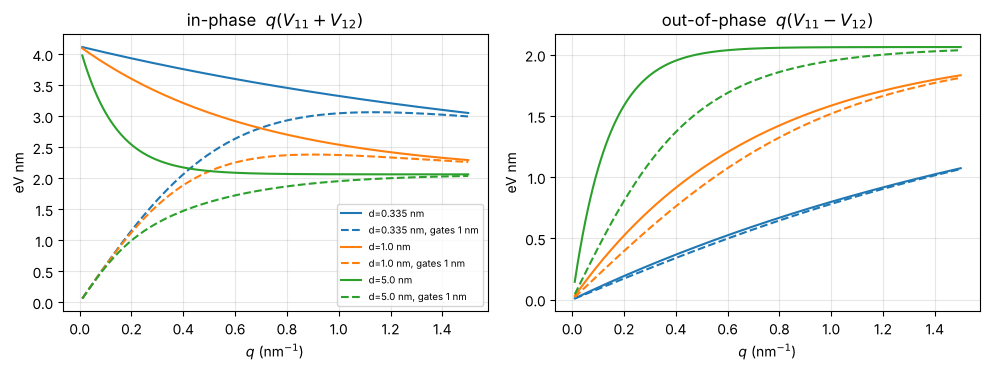
\includegraphics[width=0.92\textwidth]{figures/fig_coulomb_channels.png}
\caption{In-phase and out-of-phase Coulomb channels $q(V_{11}\pm V_{12})$ of two sheets in hBN
($\varepsilon_\parallel=6.41$, $\varepsilon_z=3$) for three separations, without (solid) and with (dashed) gates 1 nm
away. Without gates $qV_+\to4\pi e^2/\bar\varepsilon=4.13$ eV\,nm at $q\to0$ and both tend to $2\pi e^2/\bar\varepsilon$ at
$q\gg1/d$; the out-of-phase channel vanishes linearly, $qV_-\simeq2\pi e^2qd/\varepsilon_z$. Gates kill the long-range
in-phase part and barely touch the out-of-phase one.}
\label{fig:channels}
\end{figure}

The closed forms of \cref{sec:electrostatics} are reproduced to machine precision (e.g.\ $V_{12}/V_{11}=e^{-\kappa d}=0.8634$
at $d=0.335$ nm), the dispersive hBN kernel is passive in the Reststrahlen bands, and the capped-slab kernel
interpolates between its limits (\cref{fig:channels}).

\subsection{Doped monolayer graphene (notebook 02)}

The SLG$|$1 nm hBN$|$SLG junction with $n=10^{12}$ cm$^{-2}$ in both sheets ($k_F=0.177$ nm$^{-1}$, $E_F=116.6$ meV,
$\bar\varepsilon=4.39$, graphene fine-structure constant $e^2/\bar\varepsilon\hbar v_F=0.50$). The closed-form $\chi^0$ agrees with
a brute-force Lindhard sum to $<6\times10^{-3}D(E_F)$.

\begin{figure}[htbp]
\centering
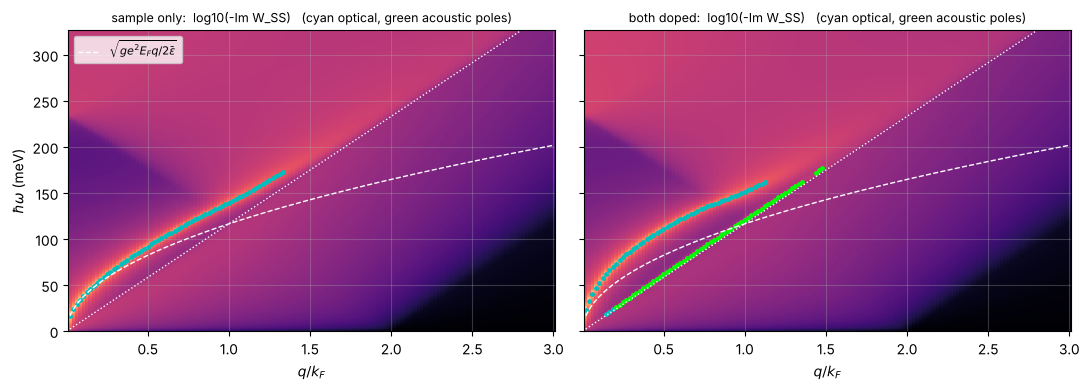
\includegraphics[width=\textwidth]{figures/fig_slg_plasmons.png}
\caption{Loss $\log_{10}(-\Imm W_{SS})$ of the sample sheet with the plasmon poles found as minima of
$|\lambda_{\min}(\varepsilon)|$. Left: inert tip, one optical branch following $\sqrt{ge^2E_Fq/2\bar\varepsilon}$ (dashed) at small
$q$. Right: both sheets doped, an additional acoustic branch (green) with $v_{\rm ac}/v_F=1.048$, above the
intraband continuum edge $\omega=v_Fq$ (dotted) as it must be. Both branches enter the continuum and stop being
poles; at 53\% of the $q$ points there is no pole at all.}
\label{fig:slgplasmons}
\end{figure}

\begin{figure}[htbp]
\centering
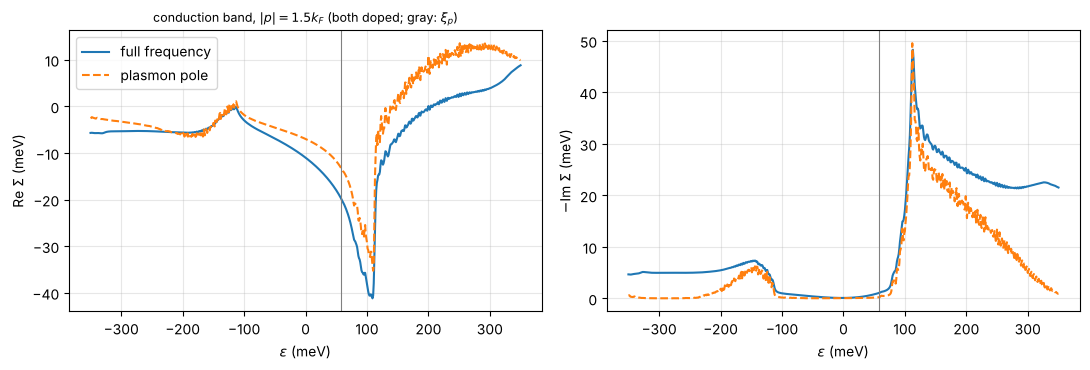
\includegraphics[width=\textwidth]{figures/fig_slg_sigma.png}
\caption{$\Sigma$ of the conduction band at $|\bp|=1.5k_F$ (bare energy $\xi_{\bp}=58$ meV, gray). Full frequency (solid)
vs plasmon-pole approximation (dashed). The PPA reproduces the plasmon-emission threshold at $\eps\simeq110$ meV but
misses the continuum contribution to $-\Imm\Sigma$ at high energy and the associated part of $\Ree\Sigma$; its ripples
come from the discrete set of poles $(\bq,\omega_n(\bq))$ on the $q$ grid.}
\label{fig:slgsigma}
\end{figure}

\begin{figure}[htbp]
\centering
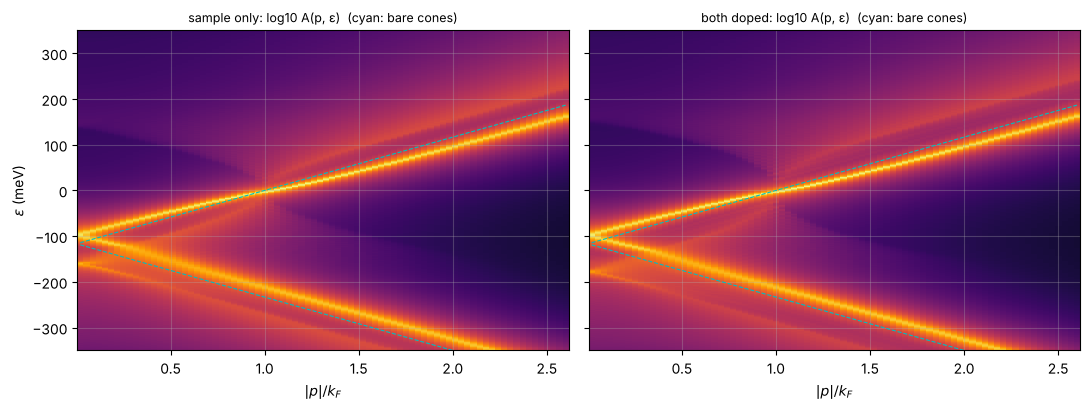
\includegraphics[width=\textwidth]{figures/fig_slg_spectral.png}
\caption{$\log_{10}A(|\bp|,\eps)$ of the sample, inert tip (left) and doped tip (right); cyan: bare cones. The
quasiparticle bands are flattened by the correlation self-energy ($v^*/v_F=0.92$, $Z\simeq0.82$--$0.83$); the faint
replica bands displaced away from $E_F$ are the plasmaron satellites, the strongest one below the Dirac point at
small $|\bp|$. At $|\bp|=1.33k_F$ the window $\pm350$ meV holds 98.8\% of the spectral weight.}
\label{fig:slgspectral}
\end{figure}

\begin{figure}[htbp]
\centering
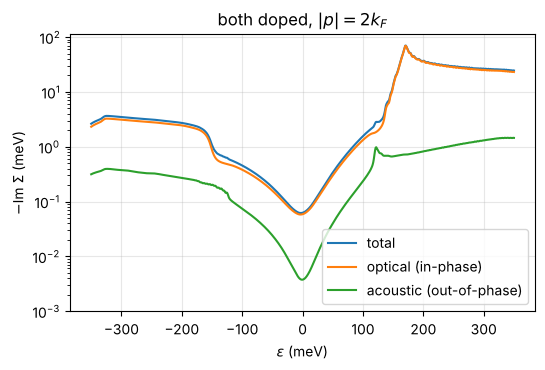
\includegraphics[width=0.55\textwidth]{figures/fig_slg_channels.png}
\caption{Layer-channel decomposition (\cref{eq:channels}) of $-\Imm\Sigma$ at $|\bp|=2k_F$, both sheets doped. The split
is exact (additivity $10^{-15}$); the acoustic (out-of-phase) channel carries $\simeq4\%$ of $\|\Sigma\|$.}
\label{fig:slgchannels}
\end{figure}

The kernel route reproduces the direct frequency integration to $1.3\times10^{-4}$ (1.1 s against 78 s per
$\bk$). The plasmaron satellites of \cref{fig:slgspectral} are the features probed by the QTM in
\cref{sec:resqtmslg}; the acoustic plasmon of the junction contributes little to the sample self-energy at a 1 nm
spacing because its weight in $W_{SS}$ is small: the out-of-phase Coulomb channel $V_-\propto d$ is weak
(\cref{sec:channelsV,fig:slgchannels}).

\subsection{Twisted bilayer graphene (notebook 03)}

\begin{figure}[htbp]
\centering
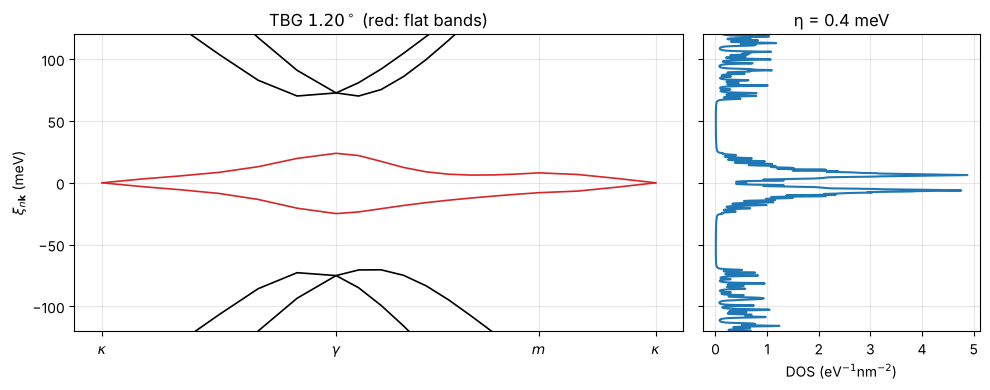
\includegraphics[width=0.9\textwidth]{figures/fig_tbg_bands.png}
\caption{Continuum bands of TBG at $1.20^\circ$ ($u_{AB}=117$ meV, $u_{AA}=0.7u_{AB}$) along $\kappa$--$\gamma$--$m$--$\kappa$ of the
$18\times18$ mesh, and density of states. Flat bands (red): widths $24.9$ and $23.9$ meV, gaps of $44$ and $45.5$ meV to
the remote bands, chemical potential $\mu=+1.8$ meV at neutrality.}
\label{fig:tbgbands}
\end{figure}

\begin{figure}[htbp]
\centering
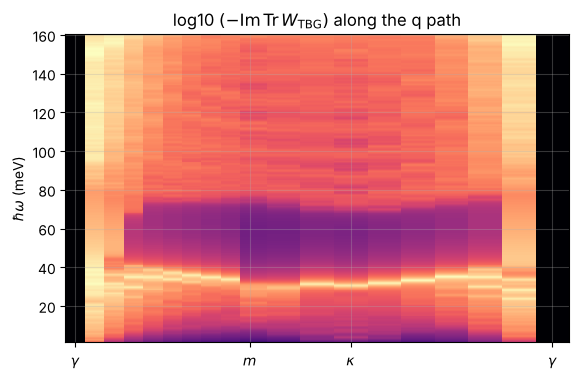
\includegraphics[width=0.62\textwidth]{figures/fig_tbg_loss.png}
\caption{Loss function $\log_{10}(-\Imm\Tr W_{\rm TBG})$ of the two TBG sheets in the SLG\,$|$\,1 nm hBN\,$|$\,TBG stack
(neutral tip), along $\gamma$--$m$--$\kappa$--$\gamma$ ($\bq=0$ is excluded, black), with the valley-summed $\chi^0$ of
\cref{eq:valleysym}. The nearly flat branch at $30$--$40$ meV is the flat-band plasmon, which lies in the gap between the intra-flat-band and
the flat-to-remote particle--hole continua~\cite{Wei2025}.}
\label{fig:tbgloss}
\end{figure}

\begin{figure}[htbp]
\centering
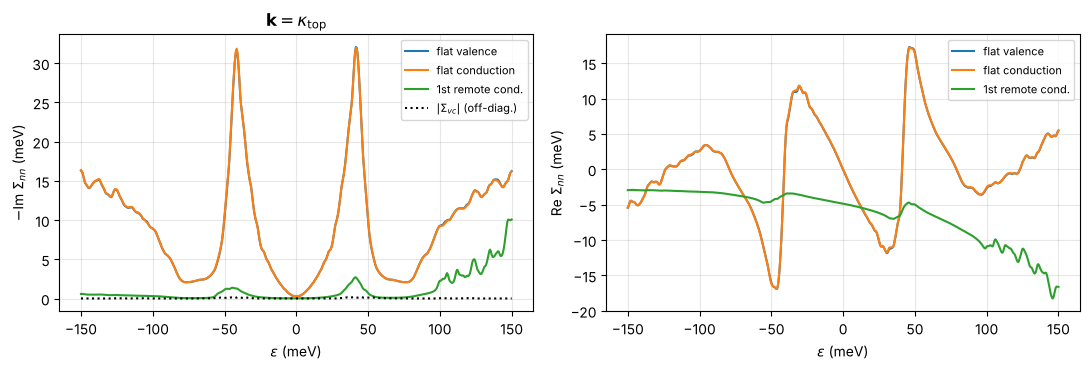
\includegraphics[width=\textwidth]{figures/fig_tbg_sigma.png}
\caption{Band-matrix G$_0$W self-energy at $\bk=\kappa_{\rm top}$ (diagonal elements; dotted: an off-diagonal element
between the two flat bands, which are degenerate at $\kappa$). The peaks of $-\Imm\Sigma$ of the flat bands at
$\eps\simeq\pm42$ meV are plasmon emission, $\eps\simeq\xi_{\rm flat}\pm\omega_{\rm pl}$; $\Ree\Sigma$ follows by
Kramers--Kronig. Kernel and direct contraction agree to $7\times10^{-5}$; $\Sigma$ is passive.}
\label{fig:tbgsigma}
\end{figure}

\begin{figure}[htbp]
\centering
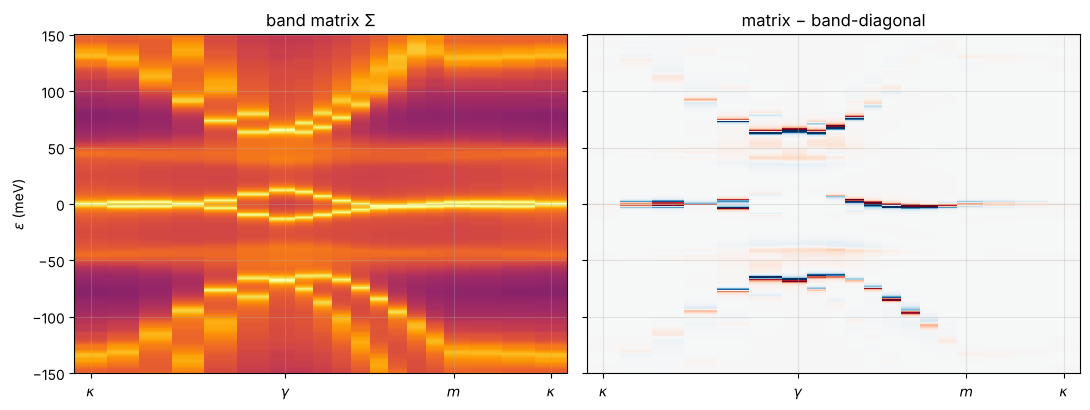
\includegraphics[width=\textwidth]{figures/fig_tbg_spectral.png}
\caption{Left: $\log_{10}\Tr A(\bk,\eps)$ from the matrix Dyson equation ($\eta_{\rm qp}=1$ meV) along
$\kappa$--$\gamma$--$m$--$\kappa$. Bright lines: quasiparticle bands; the faint, nearly $\bk$-independent lines at
$\simeq\pm(40$--$50)$ meV are the plasmon satellites of the flat bands. Right: difference between the band-matrix and the
band-diagonal $\Tr A$; it is concentrated where bands are close (flat bands, remote bands near $\gamma$).}
\label{fig:tbgspectral}
\end{figure}

\Cref{fig:tbgbands,fig:tbgloss,fig:tbgsigma,fig:tbgspectral} show the full chain for TBG. Two features deserve
comment. (i) The satellites of the flat bands are dispersionless because both the flat-band plasmon and the
intermediate flat-band states are nearly dispersionless; they are the structure the QTM is designed to detect
(\cref{sec:qtmtbg}). (ii) The band-off-diagonal self-energy changes the spectral function only where bands lie
within $|\Sigma|$ of each other, but there the change is of order one; the band-diagonal approximation is
therefore unreliable inside the flat-band manifold and at band crossings.

\subsection{QTM on doped graphene (notebook 04)}
\label{sec:resqtmslg}

\begin{figure}[htbp]
\centering
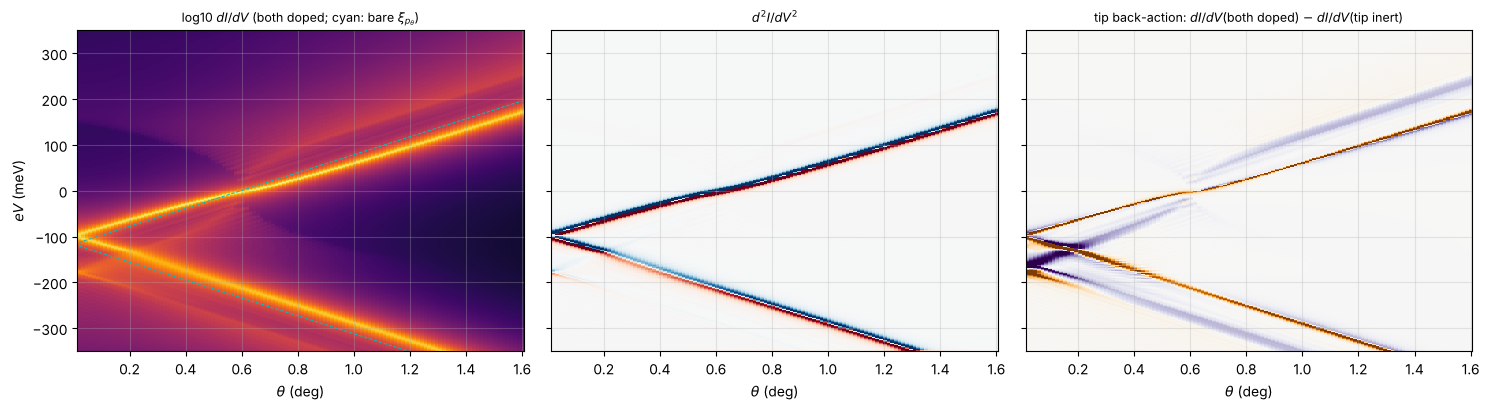
\includegraphics[width=\textwidth]{figures/fig_qtm_slg_map.png}
\caption{SLG tip\,$|$\,1 nm hBN\,$|$\,SLG sample, both at $10^{12}$ cm$^{-2}$. Left: $\log_{10}dI/dV$ from \cref{eq:didvslg}
(cyan: bare bands $\xi_{\pm}(\bp_\theta)$). Middle: $d^2I/dV^2$ after 1.5 meV Gaussian smoothing. Right: tip back-action,
the difference between a doped and an inert (non-screening) tip.}
\label{fig:qtmslgmap}
\end{figure}

\begin{figure}[htbp]
\centering
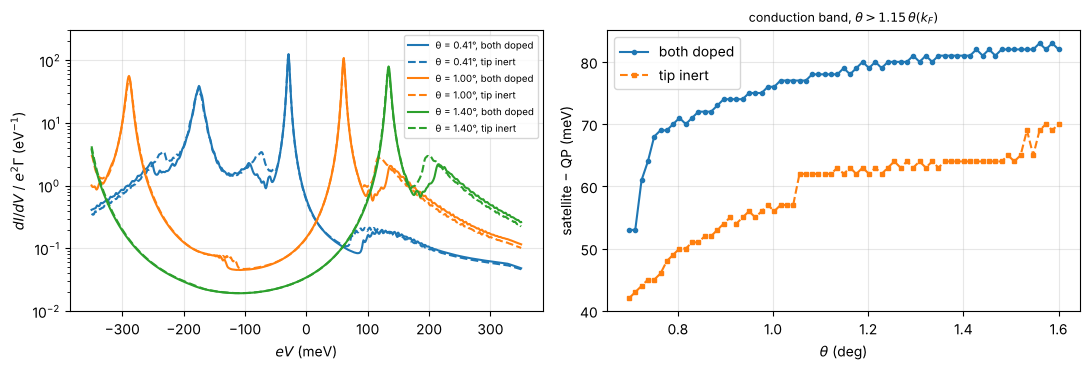
\includegraphics[width=\textwidth]{figures/fig_qtm_slg_cuts.png}
\caption{Left: line cuts of $dI/dV$ at three twist angles, doped (solid) and inert (dashed) tip. Right: offset of the
plasmaron satellite from the quasiparticle peak of the conduction band for $\theta>1.15\,\theta(k_F)$; it saturates
at $\simeq80$ meV with a doped tip and $\simeq63$ meV with an inert one.}
\label{fig:qtmslgcuts}
\end{figure}

The twist $\theta(k_F)=0.60^\circ$ brings the probed momentum to the Fermi surface, where the conduction-band ridge
crosses $eV=0$ (\cref{fig:qtmslgmap}); for $\theta\to0$ both ridges meet at the Dirac point, at $eV\simeq-100$ meV instead of $-E_F=-117$ meV because of
$\Ree\Sigma$. The chiral
matrix element changes the map by less than 0.7\% with respect to a constant one, as expected from
\cref{eq:didvslg}. The satellites run parallel to the quasiparticle ridges on the side away from $E_F$. Their
offset from the quasiparticle peak grows with $\theta$ and saturates (\cref{fig:qtmslgcuts}); doping the tip adds
its Drude weight to the in-phase plasmon of the junction and raises the offset by $\simeq17$ meV, the back-action
that a QTM with a metallic tip necessarily has. The offset is not the plasmon energy at a single momentum;
its origin and size are explained in \cref{sec:edge}.

\subsection{QTM on twisted bilayer graphene (notebook 05)}
\label{sec:resqtmtbg}

\begin{figure}[htbp]
\centering
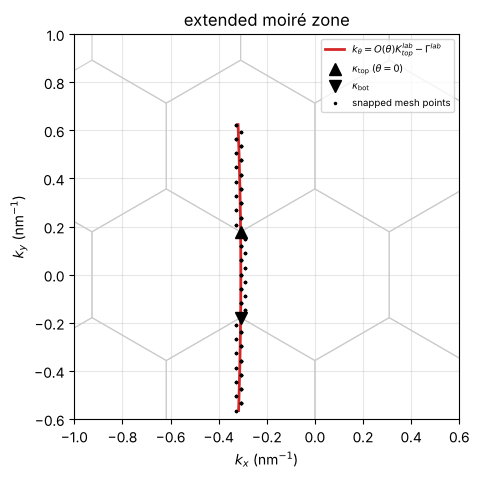
\includegraphics[width=0.48\textwidth]{figures/fig_qtm_tbg_trajectory.png}\hfill
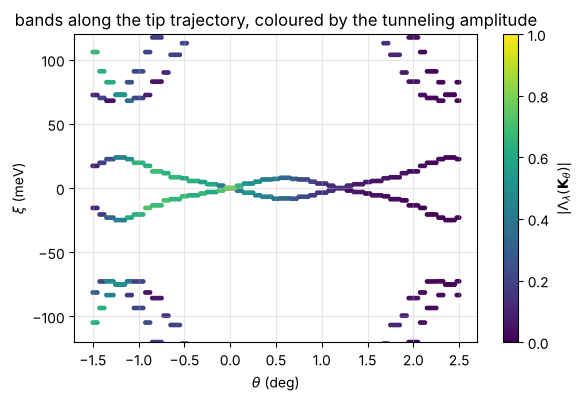
\includegraphics[width=0.5\textwidth]{figures/fig_qtm_tbg_bands.png}
\caption{Left: tip trajectory $\bk_\theta$, $\theta\in[-1.5^\circ,2.5^\circ]$, in the extended moir\'e zone (red), with the mesh
points it is snapped to. Right: the eight bands at
the snapped momenta, coloured by $|\Lambda_\lambda(\bk_\theta)|$ of \cref{eq:Lambdatbg}: near $\theta=0$ the tip sees the
flat bands through their top-layer Dirac-cone component; away from $\kappa_{\rm top}$ the weight moves out of the
computed band window.}
\label{fig:qtmtbgtraj}
\end{figure}

\begin{figure}[htbp]
\centering
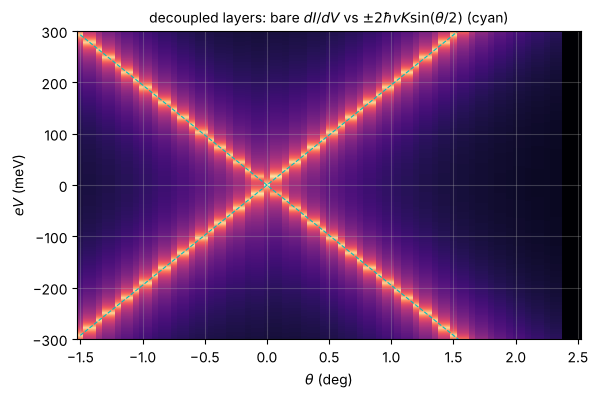
\includegraphics[width=0.62\textwidth]{figures/fig_qtm_tbg_decoupled.png}
\caption{Validation with the interlayer hopping switched off ($24\times24$ mesh, 16 bands): the bare conductance follows the
top-layer Dirac cone $eV=\pm2\hbar vK\sin(\theta/2)$ (cyan) for all $\theta$, also outside the first moir\'e zone,
because the amplitude is taken from the plane wave that unfolds the momentum (\cref{eq:Lambdatbg}). The map is dark
for $\theta\gtrsim2.4^\circ$, where $\bk_\theta$ leaves the plane-wave cutoff.}
\label{fig:qtmtbgdec}
\end{figure}

\begin{figure}[htbp]
\centering
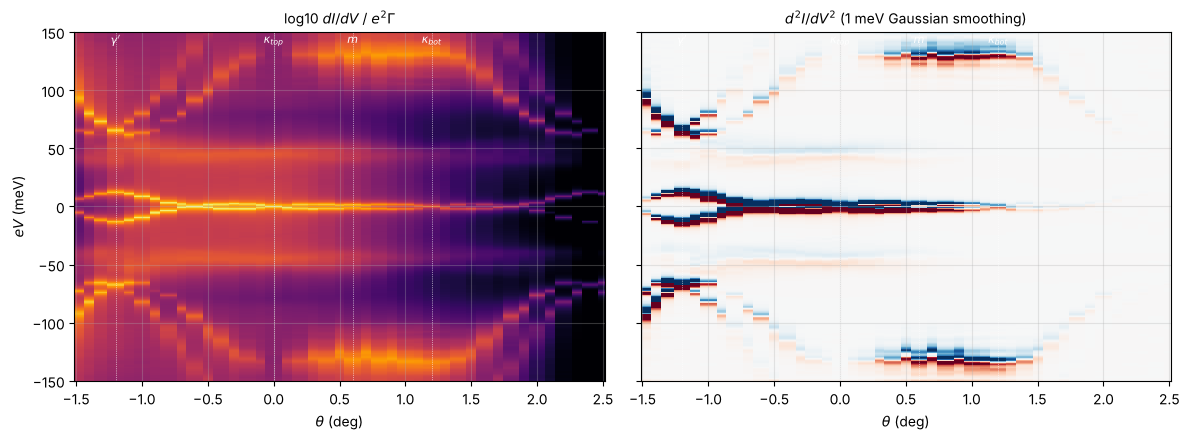
\includegraphics[width=\textwidth]{figures/fig_qtm_tbg_map.png}
\caption{$dI/dV(V,\theta)$ (left, log scale) and $d^2I/dV^2$ (right, 1 meV smoothing) of the SLG tip\,$|$\,1 nm hBN\,$|$\,TBG
junction at neutrality, from the band-matrix G$_0$W spectral function. Dotted lines: $\theta$ at which the tip probes
$\gamma'$, $\kappa_{\rm top}$, $m$ and $\kappa_{\rm bot}$. The map is piecewise constant in $\theta$ because the momentum is
snapped to the $18\times18$ mesh (36 distinct points).}
\label{fig:qtmtbgmap}
\end{figure}

\begin{figure}[htbp]
\centering
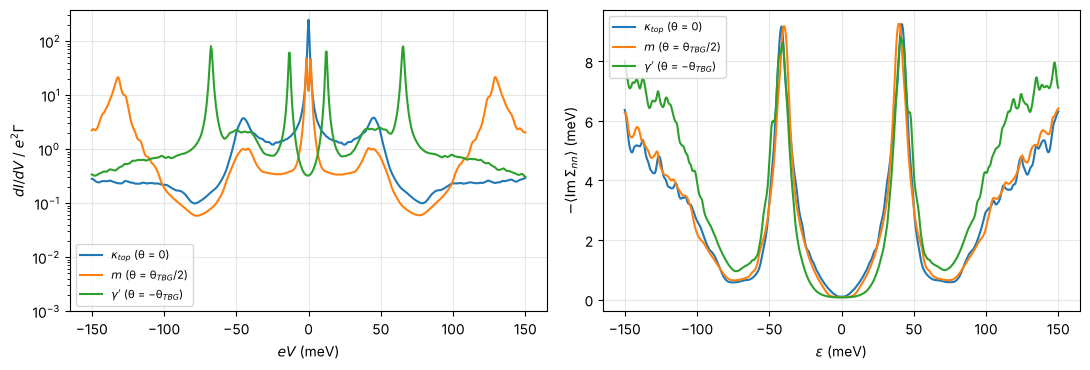
\includegraphics[width=\textwidth]{figures/fig_qtm_tbg_cuts.png}
\caption{Left: $dI/dV$ at $\kappa_{\rm top}$, $m$ and $\gamma'$. Right: band-averaged $-\Imm\Sigma_{nn}$ at the same momenta.
The quasiparticle peaks move with $\theta$; the satellites at $|eV|\simeq45$ meV do not, because they come from the
emission of the nearly dispersionless flat-band plasmon by flat-band electrons (the peaks of $-\Imm\Sigma$ at
$\pm40$ meV).}
\label{fig:qtmtbgcuts}
\end{figure}

\begin{figure}[htbp]
\centering
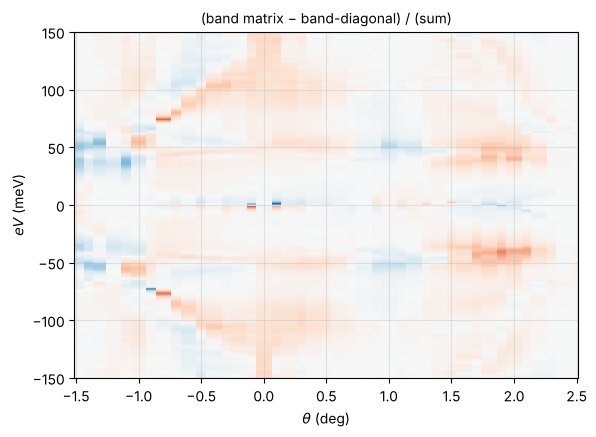
\includegraphics[width=0.62\textwidth]{figures/fig_qtm_tbg_interband.png}
\caption{Relative difference between the conductance from the band-matrix spectral function and from the
band-diagonal approximation, $(dI/dV_{\rm matrix}-dI/dV_{\rm diag})/(\text{sum})$, along the trajectory.}
\label{fig:qtmtbginterband}
\end{figure}

The physical kinematics puts the Dirac points of the two layers at $\theta=0$ and $\theta=\theta_{\rm TBG}$, where the
flat-band quasiparticle peak crosses $eV=0$, and the $\gamma$ point of the next zone at $\theta=-\theta_{\rm TBG}$, where the
flat bands are split by $\simeq25$ meV and the remote bands are visible at $\pm66$ meV
(\cref{fig:qtmtbgmap,fig:qtmtbgcuts}). The flat-band satellites appear as two horizontal stripes at
$|eV|\simeq45$ meV across the whole map; in $d^2I/dV^2$ they are weak compared with the quasiparticle edges. Beyond
$\theta\simeq1.8^\circ$ the map darkens because the top-layer weight at $\bk_\theta$ is carried by bands outside the
eight computed ones. The band-off-diagonal self-energy changes the conductance by $\simeq10\%$ in $L^2$ norm, locally
by tens of percent where bands are close (\cref{fig:qtmtbginterband}).

% ======================================================================
\section{Interpretation of the results}
\label{sec:interpretation}
% ======================================================================

This section explains what the features of the spectral functions and conductance maps of
\cref{sec:results} mean physically, and how the energy of the plasmon satellites can be estimated from
the plasmon dispersion. The numbers are produced by notebook 06 and \code{g0w.satellites}.

\subsection{What the spectral function contains}

$A(\bk,\eps)$ is the probability density for adding an electron of momentum $\bk$ at energy $\eps>0$ (or
removing one at $\eps<0$); $\int\dd\eps\,A=1$. In an interacting metal the added electron has two kinds of
final state:
\begin{itemize}
\item \textbf{the quasiparticle}: the electron dressed by a cloud of \emph{virtual} density fluctuations. It gives
the sharp peak at $E^*_{\bk}$ (\cref{sec:spectral}), with weight $Z<1$ ($Z\simeq0.82$--$0.83$ in doped graphene)
and displaced from the bare band by $\Ree\Sigma$;
\item \textbf{electron plus a real plasmon}: the electron enters by creating a plasmon $\bq$ and ends at
$\bk+\bq$. This costs $\eps=\xi_{\bk+\bq}+\omega_{\rm pl}(\bq)$, so the weight $1-Z$ is spread about one plasmon energy
away from the band. Where these final states pile up, $-\Imm\Sigma$ has a peak and $A$ a faint replica of the
band: the \emph{satellite}.
\end{itemize}
This is the electronic analogue of the phonon sidebands and shake-up satellites of photoemission, with the
plasmon in place of the phonon. Two consequences are general. The satellite of an empty state lies above the
quasiparticle peak and that of an occupied state below it: always on the side away from $E_F$. And the
satellite is not a separate particle and has no fixed energy of its own: it is the edge of a continuum, whose
position depends on the plasmon \emph{dispersion} and on the band, as quantified next. At the level of G$_0$W
only one satellite appears; replicas at multiples of the plasmon energy require higher-order (vertex or
cumulant) corrections.

\subsection{One-plasmon picture of $-\Imm\Sigma$}

Inserting the plasmon part of the spectral density, $S(\bq,\omega)\simeq R(\bq)\,\delta(\omega-\omega_{\rm pl}(\bq))$, into
the anti-Hermitian part of $\Sigma$ (\cref{sec:passivity}) gives for an empty state ($\eps>0$, $T=0$)
\begin{equation}
-\Imm\Sigma_{n}(\bk,\eps)\simeq\pi\sum_{\bq}w_{\bq}\sum_m\Theta(\xi_{m,\bk+\bq})\,
\bigl|\rho_{nm}(\bk,\bq)\bigr|^2_{R}\;\delta\bigl(\eps-E_{m\bk}(\bq)\bigr),\qquad
E_{m\bk}(\bq)=\xi_{m,\bk+\bq}+\omega_{\rm pl}(\bq),
\label{eq:onePlasmon}
\end{equation}
where $|\rho|^2_R=\sum_{ab}\rho^a_{nm}R_{ab}\rho^{b*}_{nm}$ (for graphene, the chirality factor times the residue). This
is a density of final states on the $\bq$ plane, weighted by the coupling. Like a density of states, it peaks
where the final energy $E_{m\bk}(\bq)$ is \emph{stationary} in $\bq$. The satellite energy is therefore a stationary
value of $E_{m\bk}(\bq)$, not $\omega_{\rm pl}$ at a particular $\bq$. \Cref{eq:onePlasmon} is used here only for
interpretation: all spectra of \cref{sec:results} are computed with the full spectral density of $W$, which also
contains the particle--hole continuum.

\subsection{Dispersive plasmon: the emission edge in graphene}
\label{sec:edge}

\paragraph{Estimate.} At fixed $q=|\bq|$, the direction of $\bq$ sweeps the final band energy
$\xi_{\bk+\bq}$ over $[\xi_{\bk}-\hbar v_Fq,\ \xi_{\bk}+\hbar v_Fq]$; the lowest value belongs to emission against the
electron's motion (the electron loses momentum along its velocity), and the angular density diverges at both
ends of the interval. The lower ends
\begin{equation}
E_-(q)=\xi_{\bk}+\omega_{\rm pl}(q)-\hbar v_Fq
\end{equation}
form a curve that, for a gapless 2D plasmon, first rises and then falls. At its maximum a whole range of $q$
starts contributing at the same energy (a caustic), the inverse-square-root singularities add up, and
$-\Imm\Sigma$ rises steeply. This is the emission edge:
\begin{equation}
\boxed{\eps_{\rm sat}\simeq\xi_{\bk}+\Delta,\qquad \Delta=\max_q\bigl[\omega_{\rm pl}(q)-\hbar v_Fq\bigr],\qquad
\left.\frac{d\omega_{\rm pl}}{dq}\right|_{q^*}=v_F}
\label{eq:edge}
\end{equation}
(\code{satellites.dispersive\_edge}). The maximum is reached where the plasmon group velocity equals the electron
velocity, a Cherenkov-like matching condition. The final state must be empty, $\xi_{\bk}-\hbar v_Fq^*\ge0$, i.e.
$|\bk|\ge k_F+q^*$; for smaller $|\bk|$ the edge is cut by Pauli blocking. For occupied states the mirror construction
gives $\eps_{\rm sat}\simeq\xi_{\bk}-\Delta$ for $|\bk|\le k_F-q^*$. Below the edge only small $q$ (small weight $w_qR$)
and large $q$ (Landau-damped plasmon) contribute, which is why $-\Imm\Sigma$ is small there.

\paragraph{Closed form.} For the long-wavelength plasmon $(\hbar\omega_{\rm pl})^2=\frac g2\frac{e^2}{\bar\varepsilon}E_Fq\equiv a^2q$,
maximising $a\sqrt q-\hbar v_Fq$ gives
\begin{equation}
q^*=\frac{a^2}{4(\hbar v_F)^2}=\frac g8\,\alpha_g\,k_F,\qquad
\Delta=\frac{a^2}{4\hbar v_F}=\frac g8\,\alpha_g\,E_F\ \stackrel{g=4}{=}\ \frac{\alpha_gE_F}{2},\qquad
\alpha_g=\frac{e^2}{\bar\varepsilon\hbar v_F}
\label{eq:edgeclosed}
\end{equation}
(\code{satellites.sqrt\_plasmon\_edge}): the satellite offset is a fraction of $E_F$ set by the graphene
fine-structure constant. For our junction ($\alpha_g=0.50$, $E_F=116.6$ meV) this gives $\Delta=29$ meV and
$q^*=0.25k_F$. The RPA plasmon of the junction lies above the $\sqrt q$ law at $q\sim0.4k_F$, and the full
dispersion gives larger values (\cref{tab:edge}).

\begin{figure}[htbp]
\centering
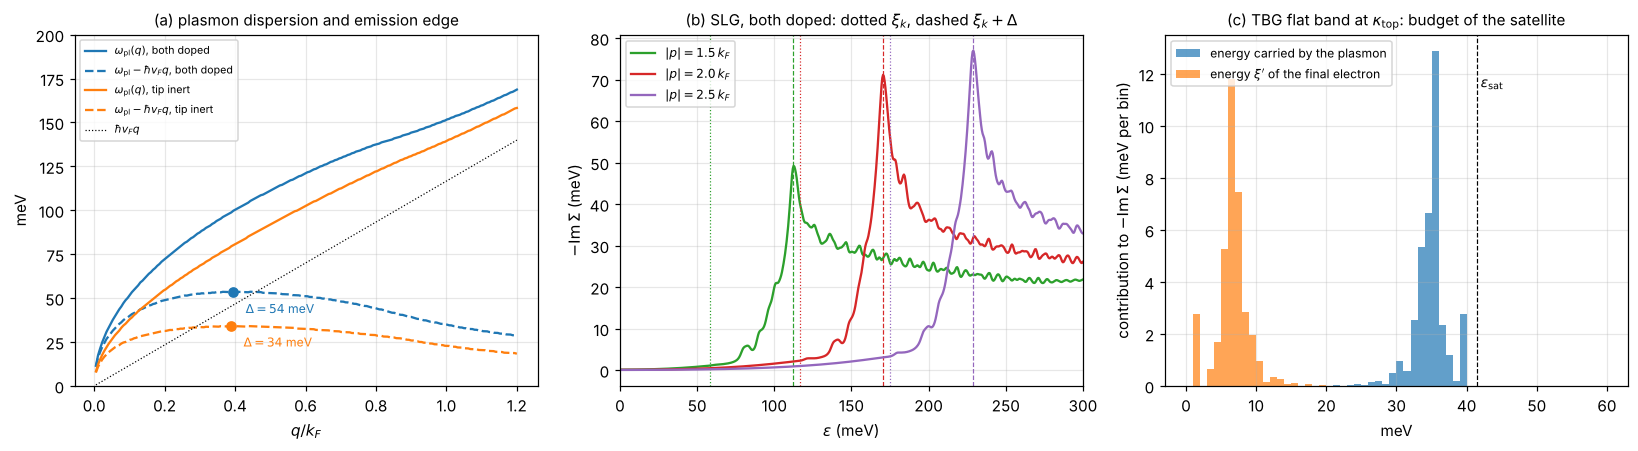
\includegraphics[width=\textwidth]{figures/fig_satellites.png}
\caption{(a) RPA plasmon dispersion of the sample sheet (solid) and $\omega_{\rm pl}(q)-\hbar v_Fq$ (dashed) for the doped and
the inert tip; dots: the maximum $\Delta$ of \cref{eq:edge}. (b) Full-frequency $-\Imm\Sigma$ of the conduction band at
three momenta (both sheets doped): the edge sits at $\xi_{\bk}+\Delta$ (dashed), one constant offset above the
bare band (dotted). (c) TBG, flat conduction band at $\kappa_{\rm top}$: decomposition of $-\Imm\Sigma$ at its peak
$\eps_{\rm sat}=41.5$ meV into the energy carried by the plasmon and the energy of the final electron.}
\label{fig:satellites}
\end{figure}

\begin{table}[htbp]
\centering
\small
\caption{Emission edge of the graphene sample: \cref{eq:edge} against the full-frequency calculation. All
energies in meV; $E^*$ is the quasiparticle peak of $A$.}
\label{tab:edge}
\begin{tabular}{lcccccccc}
\toprule
tip & $\Delta$ & $q^*/k_F$ & $|\bk|/k_F$ & $\xi_{\bk}$ & $\xi_{\bk}+\Delta$ & peak of $-\Imm\Sigma$ & satellite of $A$ & sat.\,$-\,E^*$\\
\midrule
doped & 53.7 & 0.40 & 1.5 & 58.3 & 112.0 & 112.5 & 115.0 & 73.0\\
      &      &      & 2.0 & 116.6 & 170.3 & 170.5 & 174.5 & 79.0\\
      &      &      & 2.5 & 174.9 & 228.6 & 229.0 & 233.0 & 82.0\\
inert & 34.1 & 0.39 & 1.5 & 58.3 & 92.4 & 92.5 & 95.5 & 53.5\\
      &      &      & 2.0 & 116.6 & 150.7 & 151.0 & 157.5 & 62.5\\
      &      &      & 2.5 & 174.9 & 209.0 & 209.0 & 215.0 & 64.5\\
\bottomrule
\end{tabular}
\end{table}

\paragraph{Check.} \Cref{eq:edge} reproduces the peak of the full-frequency $-\Imm\Sigma$ to within 0.5 meV at every
momentum (\cref{tab:edge,fig:satellites}b), and the plasmon slope at $q^*$ equals $v_F$ to 2\%. The satellite peak of $A$ lies
2--7 meV higher, pushed by the Dyson denominator $(\eps-\xi_{\bk}-\Ree\Sigma)^2$ of \cref{eq:Ascalar}.

\paragraph{Energy budget.} Neither $\omega_{\rm pl}(q^*)$ ($\simeq100$ meV) nor $\Delta$ ($\simeq54$ meV) is the energy of the emitted
plasmon. Decomposing $-\Imm\Sigma$ at the edge into the energy $\omega=\eps-\xi'$ carried away by the plasmon and the
energy $\xi'$ of the final electron (\code{satellites.slg\_energy\_loss}, $\eta\to0$): at $|\bk|=1.5k_F$ the plasmon
carries on average 82 meV (inter-quartile range 67--100 meV) and the electron ends at $\xi'\simeq30$ meV, with
momentum transfers around $0.3k_F$; at $2k_F$ the numbers are 96 meV (77--115 meV) and $\xi'\simeq75$ meV. The energy
of the added electron is shared between the plasmon and the drop of the electron's own band energy.

\paragraph{Offset seen in a QTM line cut.} A line cut measures the satellite relative to the quasiparticle peak,
\begin{equation}
\eps_{\rm sat}-E^*_{\bk}\simeq\Delta+\bigl(\xi_{\bk}-E^*_{\bk}\bigr)+\delta_D ,
\label{eq:offset}
\end{equation}
where $\xi_{\bk}-E^*_{\bk}=-\Ree\Sigma$ at the quasiparticle (16, 21 and 24 meV at $|\bk|=1.5$, 2 and $2.5k_F$) and
$\delta_D\simeq2$--$7$ meV is the Dyson shift. This accounts for the offsets of \cref{fig:qtmslgcuts}:
\begin{itemize}
\item \textbf{Plateau.} $\Delta$ does not depend on $\bk$, so the offset grows only through the slowly increasing
$-\Ree\Sigma$ and is nearly constant at large $\theta$: $\simeq80$ meV with a doped tip, $\simeq63$ meV with an inert one.
\item \textbf{Onset.} The edge needs $|\bk|\ge k_F+q^*\simeq1.4k_F$, i.e.\ $\theta\gtrsim1.4\,\theta(k_F)=0.83^\circ$
(\cref{eq:ptheta}); below that the edge is Pauli-blocked and the offset is smaller, as in the rising part of the
curve.
\item \textbf{Tip back-action.} Doping the tip raises $\Delta$ from 34.1 to 53.7 meV; together with the slightly
larger Dyson shift of the inert case this gives the 17 meV increase of the QTM offset. The tip's carriers oscillate in phase with the sample's in the optical
plasmon of the junction, adding Drude weight and stiffening its dispersion (in the limit $qd\to0$ the in-phase
mode of two identical sheets has twice the Drude weight, $a^2\to2a^2$, which would double $\Delta$; at $q^*$ the
computed ratio is 1.57). The satellite energy therefore depends on the electrostatic environment of the
sample, including the probe.
\end{itemize}
Because $\Sigma$ contains only the correlation part (\cref{sec:exchange}), the quasiparticle shift in
\cref{eq:offset} is correlation-only; the Fock term would move $E^*$ but not $\eps_{\rm sat}$.

\subsection{Flat plasmon and flat bands: twisted bilayer graphene}
\label{sec:flatsat}

In TBG at $1.2^\circ$ both the plasmon and the final states are nearly dispersionless: the peak of the sample
spectral density is at $34.2$ meV over the whole moir\'e mesh (inter-quartile range 32.7--35.2 meV), and the flat bands
are $\simeq25$ meV wide. The $\bq$ integral then hardly matters, and the stationary value of $E_{m\bk}(\bq)$ is reached
where the density of final flat-band states peaks, at the van Hove energy $\xi_{\rm VH}$:
\begin{equation}
\boxed{\eps_{\rm sat}\simeq\pm\bigl(\xi_{\rm VH}+\bar\omega_{\rm pl}\bigr)}
\label{eq:flatsat}
\end{equation}
With $\xi_{\rm VH}=6.2$ meV (peak of the conduction flat-band DOS) this gives 40.5 meV, against the computed peak of
$-\Imm\Sigma$ of the flat band at $\kappa_{\rm top}$, 41.5 meV. The decomposition (\code{satellites.tbg\_energy\_loss},
\cref{fig:satellites}c) confirms the picture: the plasmon carries $34.8$ meV on average (inter-quartile range
33.8--35.6 meV) and all final states lie in the flat band, at $\xi'\simeq6.7$ meV. The satellite of $A$ and of
$dI/dV$ appears at $|eV|\simeq45$ meV, again a few meV beyond the peak of $-\Imm\Sigma$ because of the Dyson
denominator. The hole satellite is the mirror image, by the approximate particle--hole symmetry of the
continuum bands.

Since neither $\bar\omega_{\rm pl}$ nor $\xi_{\rm VH}$ depends on $\bk$, the satellite energy is the same at every momentum
probed by the tip. This is why, in \cref{fig:qtmtbgmap,fig:qtmtbgcuts}, the satellites form horizontal stripes
that do not move with the twist angle, while the quasiparticle peaks follow the bands along the trajectory
(zero bias at $\kappa_{\rm top}$ and $\kappa_{\rm bot}$, $\pm12$ meV at $\gamma'$). The angle independence is the
fingerprint that distinguishes a flat-plasmon satellite from a band.

\subsection{What a QTM measurement of the satellites determines}

Since $dI/dV\propto\bra{\chi_\theta}A(\bK_\theta,eV)\ket{\chi_\theta}$ (\cref{eq:didv}), the quasiparticle ridges of a map give the
renormalised bands and the satellites give the one-plasmon emission edges. In graphene the satellite
offset is not the plasmon energy but $\Delta=\max_q[\omega_{\rm pl}-\hbar v_Fq]$, a property of the plasmon dispersion
near the momentum where its slope equals $v_F$, plus the quasiparticle shift of \cref{eq:offset}; extracting
plasmon information from it requires either the measured quasiparticle ridge and band velocity, or the
calculation. In flat-band TBG the offset is close to $\bar\omega_{\rm pl}+\xi_{\rm VH}-E^*_{\bk}$, a nearly direct, angle-independent
measure of the flat-band plasmon energy. In both cases the edge is sharpened in $d^2I/dV^2$, and its position
depends on the screening environment, the tip included.

% ======================================================================
\section{Numerics, validation and limitations}
\label{sec:numerics}
% ======================================================================

\subsection{Grids and broadenings}

\begin{center}
\small
\begin{tabularx}{\textwidth}{lXX}
\toprule
& SLG $|$ hBN $|$ SLG (notebooks 02, 04) & SLG $|$ hBN $|$ TBG (notebooks 03, 05)\\
\midrule
momenta $\bq$ & radial, $n_q=144$ (02), $96$ (04) on $[0.02,3]k_F$; $n_\theta=64$ angles & $18\times18$ moir\'e mesh (324 points), $\bq=0$ removed\\
bands & two Dirac bands, analytic & $8$ continuum bands, $G_{\max}=3$ (37 plane-wave shells)\\
$\omega$ grid for $S$ & $480$ points on $[10^{-4},2.8E_F]$ & $320$ points on $[2\eta,160\ \text{meV}]$\\
$\eta$ ($\chi^0$, $V$, $W$) & 1 meV & $0.71$ meV $=2v_n|\bG_M|/N_s$\\
$\eta_\Sigma$ (resolvents) & 1 meV & $=\eta$\\
$\eta_{\rm qp}$ (Dyson) & 2 meV & 0.5 meV\\
$\eps$ grid ($=eV$) & 701 points on $\pm350$ meV & 601 points on $\pm150$ meV\\
kernel step $du$ & $\eta_\Sigma/8$ & $\eta_\Sigma/8$\\
\bottomrule
\end{tabularx}
\end{center}

\paragraph{Three broadenings, three roles.} $\eta$ turns the undamped collective modes into Lorentzians that the
$\omega$ grid can integrate; it must exceed the grid step and, for TBG, the mesh floor $v_n|\bG_M|/N_s$ below which
$\chi^0$ resolves individual $\bk$ points (\code{TBGParams.eta\_mesh}). $\eta_\Sigma$ regularises the resolvents of
\cref{eq:sigma}; it sets the energy resolution of $\Sigma$ and the floor of $-\Imm\Sigma$ at $\eps=0$. $\eta_{\rm qp}$ is
an extrinsic width added in the Dyson equation; it keeps $A$ finite where $\Imm\Sigma\to0$ and plays the role of
the experimental resolution. Physical widths are those of $-\Imm\Sigma$ that exceed all three.

\paragraph{Away from the magic angle.} The TBG heuristic $\eta=2v_n|\bG_M|/N_s$ scales with the renormalised
velocity; at $5^\circ$ it gives $\sim120$ meV and must be replaced by \code{eta\_override}.

\subsection{Cost}

The TBG pipeline of notebook 03 on one CPU core: band structure 10 s; form factors $\rho^\ell_{nm}(\bk,\bq)$ 35 s
(0.21 GB for $2\times8\times8\times324\times324$); $\chi^0$ and $W$ on $324\times320$ $(\bq,\omega)$ points 39 s; resolvent
kernel 4 s; band-matrix $\Sigma$ ($8\times8\times601$) $\simeq1$ s per $\bk$ with the kernel against $\simeq12$ s for the
direct contraction. The direct route scales as $n_q\,n_\omega\,n_b^2\,n_m\,n_\eps$, the kernel route as
$n_q\,n_b^2\,n_m\,n_\eps$ after a one-off tabulation of cost $n_q\,n_\omega\,n_u$. For SLG the kernel route costs $\simeq1$--$2$ s per $(\bk,\text{band})$ with $n_q=96$--$144$ and $n_\vartheta=64$, against
$\simeq80$ s for the direct integration. Memory is dominated by
\code{densityL}, which grows as $N_s^4$: $N_s=24$ needs $0.7$ GB and $N_s=30$ 1.7 GB.

\subsection{Validation}

The test suite (\code{python tests/run\_tests.py}, 42 tests, $\sim$1.5 min) checks:

\begin{center}
\small
\begin{tabularx}{\textwidth}{Xl}
\toprule
check & result\\
\midrule
$V$ of 1 and 2 sheets, gated and ungated, against closed forms (\cref{sec:electrostatics}) & $<10^{-6}$ relative\\
capped-slab limits; gate suppresses the in-phase channel more than the out-of-phase one & exact limits\\
$(\ell,\bG)$ flattening identical in $\varepsilon$ and $V$ & exact\\
closed-form graphene $\chi^0$ vs brute-force Lindhard sum ($1000\times1000$ polar grid) & $<2\times10^{-3}D(E_F)$\\
$\chi^0(q\to0,0)=-D(E_F)$; $\Imm\chi^0\le0$ for $\omega>0$ & yes\\
fast TBG $\chi^0$ vs \texttt{pybandstructure} \code{polarization} & $3\times10^{-15}$\\
TBG $\chi^0$ and $W$ obey the Onsager relation $X(\bq)=X(-\bq)^T$ & $5\times10^{-16}$\\
$\sum_\ell\rho^\ell_{nm}(\bk,0)=\delta_{nm}$ & $10^{-14}$\\
band-matrix $\Sigma$: diagonal equals the independent band-diagonal routine & $4\times10^{-16}$\\
kernel route vs direct contraction (SLG, TBG; notebooks 02, 03) & $1.3\times10^{-4}$, $7\times10^{-5}$\\
$\Sigma$ passive ($(\Sigma-\Sigma^\dagger)/2\ii\preceq0$), gauge covariant & yes\\
$\int\Tr A=n_b$ for $\Sigma=0$; Dyson root and $Z$ for linear $\Sigma$ & $10^{-3}$; exact\\
channel split of $W$ and $\Sigma$ is additive & $10^{-15}$\\
TBG flat bands at $1.20^\circ$; model-frame Dirac points; eigenvector order & yes\\
tip trajectory through $\kappa_{\rm top}$, $\kappa_{\rm bot}$, $\gamma'$; snapping $\le1/\sqrt3$ spacing & yes\\
decoupled layers: bare $dI/dV$ follows $\pm2\hbar vK\sin(\theta/2)$ & within 1.5 meV\\
band-matrix $dI/dV$ gauge invariant and $\ge0$ & yes\\
emission edge of a $\sqrt q$ plasmon equals \cref{eq:edgeclosed}; slope $v_F$ at $q^*$ & $10^{-6}$; 1\%\\
energy-loss decomposition sums to the full-frequency $-\Imm\Sigma$ & $<5\%$\\
\bottomrule
\end{tabularx}
\end{center}

\subsection{Limitations}

\begin{itemize}[leftmargin=*]
\item \textbf{Head only.} Local fields are omitted (\cref{as:head}). For TBG at $1.2^\circ$ the moir\'e umklapp
$\bG\neq0$ components of $\chi^0$ are not negligible at $|\bq|\sim|\bG_M|$; \code{LayerHelpers} supports $n_G>1$ for
$\chi^0$ and $\varepsilon$, but the self-energy routines contract only the head.
\item \textbf{No exchange.} \Cref{sec:exchange}: correlation-only $\Sigma$; for TBG at neutrality this matches the
scheme of Ref.~\cite{Wei2025}, for doped graphene it misses the velocity enhancement.
\item \textbf{Truncations.} For SLG, $q\le3k_F$: the large-$q$ interband tail of $W$ is cut off, which mainly affects
$\Ree\Sigma$ (logarithmically) and hence $v^*$; satellites, which come from $q\lesssim k_F$, are converged. For TBG,
$\omega\le160$ meV and $8$ bands: transitions to and between remote bands above this window are missing in $S$; their
effect on the flat bands is a nearly static real shift.
\item \textbf{Mesh.} The TBG $\bq$ sum is a $18\times18$ (or $12\times12$ for quick runs) mesh; $\Sigma$ inherits the
mesh ripples of $\chi^0$ unless $\eta\gtrsim\eta_{\rm mesh}$, and the QTM trajectory is snapped to the mesh,
so the $(\theta,V)$ map is piecewise constant in $\theta$ on steps of $|\bG_M|/(N_sK)$ ($0.12^\circ$ for $N_s=18$).
\item \textbf{Band window.} Only the 8 computed bands enter $A^S$; at large $|\theta|$ the tip probes momenta far from
$\kappa_{\rm top}$ where the top-layer weight is carried by bands outside the window, and the map darkens.
\item \textbf{Static dielectrics.} hBN is used with its static anisotropic constants unless a dispersive model from
\code{g0w.dielectrics} is chosen; phonon polaritons of hBN then enter $V(\bq,\omega)$ but are untested in the
self-energy routines.
\item \textbf{QTM.} \Cref{eq:didv} assumes perfect momentum resolution and a constant tip DOS
(\cref{sec:qtm}); temperature and lock-in broadening are mimicked by Gaussian smoothing.
\end{itemize}

\appendix
% ======================================================================
\section{Polarisability of doped graphene in closed form}
\label{app:dirac}
% ======================================================================

At $T=0$ and electron density $n$ ($k_F=\sqrt{4\pi n/g}$), with $D_\pm=(\omega/\hbar v_F\pm2k_F)/q$ and
$s=\sqrt{\omega^2-(\hbar v_Fq)^2}$ (principal root), the retarded bubble of \cref{eq:chi0} for one sheet
is~\cite{Wunsch2006}
\begin{gather}
\chi^0(q,\omega)=-\frac{g}{16\pi}\Bigl[\frac{8k_F}{\hbar v_F}+\frac{q^2}{s}\bigl(\mathcal G(D_-)+\ii\pi-\mathcal G(D_+)\bigr)\Bigr],\nonumber\\
\mathcal G(z)=z\sqrt{z-1}\sqrt{z+1}-\log\bigl(z+\sqrt{z-1}\sqrt{z+1}\bigr)
\end{gather}
(\code{dirac\_chi.chi\_dirac\_phys}). The split root makes $\mathcal G$ analytic on $\mathbb C\setminus[-1,1]$, which is the
cut structure of the retarded response, so the same expression is valid at real $\omega+\ii0$ and at complex
$\omega+\ii\eta$. No branch switch is needed: $\mathcal G(-z)=\mathcal G(z)+\ii\pi$ in the upper half plane, so the
two forms $\mathcal G(-D_-)$ and $\mathcal G(D_-)+\ii\pi$ that appear in the literature are the same analytic function
there (checked to $3\times10^{-14}$). Limits: $\chi^0(q\to0,0)=-D(E_F)$
with $D(E_F)=gk_F/(2\pi\hbar v_F)$; for $\omega\ll\hbar v_Fq$ and $q\ll k_F$ the static Thomas--Fermi form; for $q\ll k_F$
and $\omega\gg\hbar v_Fq$ the Drude form $\chi^0\simeq D(E_F)\,(\hbar v_Fq)^2/2\omega^2$, which with
$V=2\pi e^2/\bar\varepsilon q$ gives the optical plasmon
$\omega_{\rm pl}^2=\frac{g}{2}\frac{e^2}{\bar\varepsilon}E_Fq$ (\code{test\_optical\_plasmon\_long\_wavelength\_law}).
The intrinsic (undoped) part $\chi^0=-\frac{g}{16}q^2/\sqrt{(\hbar v_Fq)^2-\omega^2}$ is used for a neutral tip.


\begin{thebibliography}{99}
\bibitem{Wei2025} N.~Wei, F.~Guinea, F.~von Oppen, and L.~I.~Glazman, \emph{Theory of plasmon spectroscopy with the quantum twisting microscope}, Phys.~Rev.~B \textbf{112}, 155157 (2025).
\bibitem{Wei2025b} N.~Wei, F.~von Oppen, and L.~I.~Glazman, \emph{Dirac-point spectroscopy of flat-band systems with the quantum twisting microscope}, Phys.~Rev.~B \textbf{111}, 085128 (2025).
\bibitem{Inbar2023} A.~Inbar \emph{et al.}, \emph{The quantum twisting microscope}, Nature \textbf{614}, 682 (2023).
\bibitem{BM2011} R.~Bistritzer and A.~H.~MacDonald, \emph{Moir\'e bands in twisted double-layer graphene}, PNAS \textbf{108}, 12233 (2011).
\bibitem{Koshino2018} M.~Koshino \emph{et al.}, \emph{Maximally localized Wannier orbitals and the extended Hubbard model for twisted bilayer graphene}, Phys.~Rev.~X \textbf{8}, 031087 (2018).
\bibitem{Novelli2020} P.~Novelli, I.~Torre, F.~H.~L.~Koppens, F.~Taddei, and M.~Polini, \emph{Optical and plasmonic properties of twisted bilayer graphene: impact of interlayer tunneling asymmetry and ground-state charge inhomogeneity}, Phys.~Rev.~B \textbf{102}, 125403 (2020) [\texttt{pybandstructure}].
\bibitem{Cavicchi2024} L.~Cavicchi, I.~Torre, P.~Jarillo-Herrero, F.~H.~L.~Koppens, and M.~Polini, \emph{Theory of intrinsic acoustic plasmons in twisted bilayer graphene}, Phys.~Rev.~B \textbf{110}, 045431 (2024).
\bibitem{Wunsch2006} B.~Wunsch, T.~Stauber, F.~Sols, and F.~Guinea, \emph{Dynamical polarization of graphene at finite doping}, New J.~Phys.~\textbf{8}, 318 (2006); E.~H.~Hwang and S.~Das Sarma, Phys.~Rev.~B \textbf{75}, 205418 (2007).
\bibitem{Mahan} G.~D.~Mahan, \emph{Many-Particle Physics}, 3rd ed.\ (Kluwer, 2000); G.~Giuliani and G.~Vignale, \emph{Quantum Theory of the Electron Liquid} (Cambridge, 2005).
\bibitem{Hedin1965} L.~Hedin, \emph{New method for calculating the one-particle Green's function with application to the electron-gas problem}, Phys.~Rev.~\textbf{139}, A796 (1965).
\bibitem{Polini2008} M.~Polini, R.~Asgari, G.~Borghi, Y.~Barlas, T.~Pereg-Barnea, and A.~H.~MacDonald, \emph{Plasmons and the spectral function of graphene}, Phys.~Rev.~B \textbf{77}, 081411(R) (2008).
\bibitem{Elias2011} D.~C.~Elias \emph{et al.}, \emph{Dirac cones reshaped by interaction effects in suspended graphene}, Nat.~Phys.~\textbf{7}, 701 (2011).
\end{thebibliography}

\end{document}
